% =====================================================================
% Drought Intelligence Explorer — Data Descriptor (Version 1.0)
% Format: Scientific Data (Nature portfolio) style manuscript
% Compile: tectonic main.tex   (or: latexmk -pdf main.tex)
% =====================================================================
\documentclass[10pt,a4paper]{article}

\usepackage[T1]{fontenc}
\usepackage[utf8]{inputenc}
\usepackage{newtxtext,newtxmath}
\usepackage{textcomp}
\usepackage[a4paper,top=2.3cm,bottom=2.6cm,left=2.4cm,right=2.4cm]{geometry}
\usepackage{graphicx}
\usepackage{booktabs}
\usepackage{tabularx}
\usepackage{array}
\usepackage{ragged2e}
\usepackage{xcolor}
\usepackage{caption}
\usepackage{titlesec}
\usepackage{enumitem}
\usepackage{microtype}
\usepackage{fancyhdr}
\usepackage{natbib}
\setcitestyle{authoryear,round}

\usepackage[colorlinks=true,linkcolor=blue!55!black,citecolor=blue!55!black,urlcolor=blue!55!black]{hyperref}

\graphicspath{{figures/}}

% --- headings: unnumbered, Nature style -------------------------------
\setcounter{secnumdepth}{0}
\titleformat{\section}{\large\bfseries}{\thesection}{0.6em}{}
\titleformat{\subsection}{\normalsize\bfseries}{\thesubsection}{0.6em}{}
\titlespacing{\section}{0pt}{14pt plus 3pt minus 2pt}{6pt}
\titlespacing{\subsection}{0pt}{10pt plus 2pt minus 2pt}{4pt}

% --- captions: "Figure 1 | text", "Table 1 | text" --------------------
\DeclareCaptionLabelSeparator{pipe}{ $|$ }
\captionsetup[figure]{labelfont=bf,labelsep=pipe,font=small,justification=justified}
\captionsetup[table]{labelfont=bf,labelsep=pipe,font=small,justification=justified,skip=4pt}

% --- header ------------------------------------------------------------
\pagestyle{fancy}
\fancyhf{}
\fancyhead[L]{\small\itshape Drought Intelligence Explorer $\cdot$ EarthArXiv preprint (manuscript version 1.3)}
\fancyhead[R]{\small\thepage}
\renewcommand{\headrulewidth}{0.3pt}

\setlength{\parskip}{2pt}
\renewcommand{\arraystretch}{1.18}

\hypersetup{
  pdftitle={Drought Intelligence Explorer: a 45-year district-level dataset of ten drought indicators for India and an open analytical platform},
  pdfauthor={Ankit Deshmukh},
}

\begin{document}

% =====================================================================
% TITLE PAGE
% =====================================================================
\begin{center}
{\footnotesize\bfseries\color{gray!60!black} DATA DESCRIPTOR \quad$\cdot$\quad MANUSCRIPT VERSION 1.3 \quad$\cdot$\quad EARTHARXIV PREPRINT}\\[10pt]
{\LARGE\bfseries Drought Intelligence Explorer: a 45-year district-level dataset of ten drought indicators for India and an open analytical platform\par}
\vspace{14pt}
{\large Ankit Deshmukh\par}
\vspace{4pt}
{\small Department of Civil Engineering, School of Technology (SoT),\\Pandit Deendayal Energy University, Gandhinagar, Gujarat, 382426, India\par}
\vspace{2pt}
{\small * Correspondence: \href{mailto:deshmukh.acad@gmail.com}{deshmukh.acad@gmail.com} \ $\cdot$ \ ORCID: \href{https://orcid.org/0000-0002-1433-3872}{0000-0002-1433-3872}\par}
\vspace{2pt}
{\small Platform: \url{https://drought.ankitdeshmukh.com} \ $\cdot$ \ Software and dataset (release 1.0.0, 2026-11-10): \url{https://github.com/anixn/drought-intelligence-explorer} \ $\cdot$ \ DOI: \href{https://doi.org/10.5281/zenodo.24113364}{10.5281/zenodo.24113364}\par}
\vspace{8pt}
\end{center}

\vspace{6pt}
\section*{Abstract}
Publicly available drought records for India rarely combine sub-national detail, multi-decadal coverage, several indicator families and a documented processing chain in one citable product. Here we present a monthly, district-level dataset of ten drought indicators covering all of India from January 1981 to December 2025, together with the open, browser-based platform that serves it. Four of the indicators are standardized z-score indices: the Standardized Precipitation Index (SPI) and the Standardized Precipitation Evapotranspiration Index (SPEI), each at 1-, 3-, 6- and 12-month accumulation windows. The other two are percentage-based indicators: a root-zone Soil Moisture Anomaly (SMA) and the Vegetation Condition Index (VCI). The dataset covers 724 administrative districts in 36 States and Union Territories and holds 3{,}715{,}048 valid district-month values. The indicators come from CHIRPS v2.0 precipitation, ERA5-Land potential evaporation and root-zone soil moisture, and MODIS MOD13A3 NDVI, extracted and aggregated by a scripted Google Earth Engine pipeline. SPI, SPEI and SMA use a fixed 1981--2020 reference period (40 years); VCI uses 2000 to the release date. Missing observations are never imputed. As a scientific consistency check, the released record reproduces documented drought episodes with the expected geography and timing (for example, every Rajasthan district is flagged in July to September 2002, and the vegetation index collapses two to three months after the 2015 Marathwada rainfall deficit). Software quality is guarded by per-fit calibration gates, a checksummed release manifest and an 82-assertion offline self-test. Every value is reproducible from public inputs and documented commands, citable through a versioned DOI (10.5281/zenodo.24113364), and analysable and exportable through the platform without an account or backend. The product is a transparent research instrument, not an operational drought declaration.

\vspace{8pt}
{\small\textbf{Keywords:} drought; Standardized Precipitation Index (SPI); Standardized Precipitation Evapotranspiration Index (SPEI); Vegetation Condition Index (VCI); soil moisture anomaly; India; Google Earth Engine; reproducible research; district-level dataset; geospatial web platform\par}

% =====================================================================
\section*{Background \& Summary}
Drought is a recurring and slowly evolving climate hazard whose impacts propagate from precipitation deficits through soil moisture and vegetation to water resources, agriculture and society. Its very definition depends on the domain of impact: the literature conventionally distinguishes meteorological, agricultural, hydrological and socio-economic drought, and each type responds to deficits on a different time scale\citep{WilhiteGlantz1985,MishraSingh2010}. Standardized indices were developed to make these different facets comparable: the Standardized Precipitation Index (SPI) converts accumulated precipitation over a chosen window into a probability-based anomaly\citep{McKee1993}, the Standardized Precipitation Evapotranspiration Index (SPEI) applies the same machinery to the climatic water balance and therefore also responds to atmospheric evaporative demand and warming\citep{VicenteSerrano2010}, and vegetation-based indices such as the Vegetation Condition Index (VCI) capture the integrated land-surface response\citep{Kogan1995}. Using several of these families together, at several accumulation windows, is the recognised way to monitor drought as a propagating phenomenon rather than as a single number, and is the approach recommended by international guidance\citep{WMOLincoln2009,SvobodaFuchs2016}.

For India, the need is acute. Rainfall is dominated by a strongly seasonal monsoon with high spatial variability, agriculture remains a major user of land and water, and drought episodes repeatedly affect large shares of the national territory\citep{GadgilGadgil2006}. Indian operational practice and international guidance both converge on standardized, multi-scale indices computed against fixed reference periods\citep{WMOLincoln2009}, and high-quality national gridded observation products exist\citep{Pai2014,Srivastava2009}. Several Indian services publish drought-relevant information. The India Meteorological Department issues operational weekly SPI and aridity-anomaly products. The National Remote Sensing Centre (ISRO) publishes a national agricultural-drought assessment based on NDVI and VCI through the Bhuvan portal. India-WRIS disseminates water-resources observations. These are operational monitoring products: they are produced for current conditions, are not distributed as reproducible district-month archives, and do not ship their processing code. A researcher who wants a multi-decadal, district-level, multi-indicator record must therefore either assemble it from global products at coarse resolution, rely on single-index products, or rebuild the entire processing chain. Web platforms that lower this barrier exist for other regions; the Great Lakes Dashboard is a documented example of a hydro-climatic dashboard published as a scientific tool\citep{Smith2016}. This contribution differs from the operational services not in timeliness but in archive depth (1981--2025), in multi-indicator families held in one consistent contract, in district-level provenance, and in end-to-end reproducibility under a versioned DOI.

This contribution fills that gap with two coupled artefacts. The first is a dataset: ten drought indicators, namely SPI-1/3/6/12, SPEI-1/3/6/12, a root-zone Soil Moisture Anomaly (SMA) and the VCI, computed monthly for 724 administrative districts and 36 States and Union Territories from January 1981 to December 2025 (VCI from February 2000, where the MODIS NDVI record begins). The ten matrices together hold 3{,}715{,}048 valid district-month values. The indicators are produced from CHIRPS v2.0 daily precipitation\citep{Funk2015}, ERA5-Land potential evaporation and volumetric soil water\citep{MunozSabater2021} and MODIS MOD13A3 NDVI\citep{Didan2015}, extracted and aggregated through a scripted Google Earth Engine pipeline\citep{Gorelick2017} whose every step is a documented, re-runnable command. Figure~\ref{fig:pipeline} summarises the production chain, including the offline reference route that can replace the Earth Engine extraction, and Figure~\ref{fig:coverage} shows the temporal coverage of the ten matrices. The strength of the contribution lies in this integration: a long district-level archive, several independent indicator families, a reproducible pipeline, transparent quality control and an open analysis environment, delivered together under one citation.

The second artefact is the Drought Intelligence Explorer, the open analytical platform that serves the dataset\citep{Deshmukh2026}. It runs entirely in the browser from static files: there is no account, no backend and no API key. It organises the analysis into four workspaces (current conditions; historical analysis; drought events; indicator propagation and relationships) plus an integrated documentation centre. Regional statistics are computed live and area-weighted, ten export products carry reproducibility headers, and the interface enforces a strict data-lineage labelling so that users always know whether they are reading original observations, derived indicators, aggregated statistics or analytical summaries. Web-based dashboards of this kind have become an established publication vehicle for hydro-climatic analysis tools\citep{Smith2016}, and this platform is designed to meet that standard of documentation and reproducibility rather than to act as an operational warning system.

\begin{figure}[t]
\centering
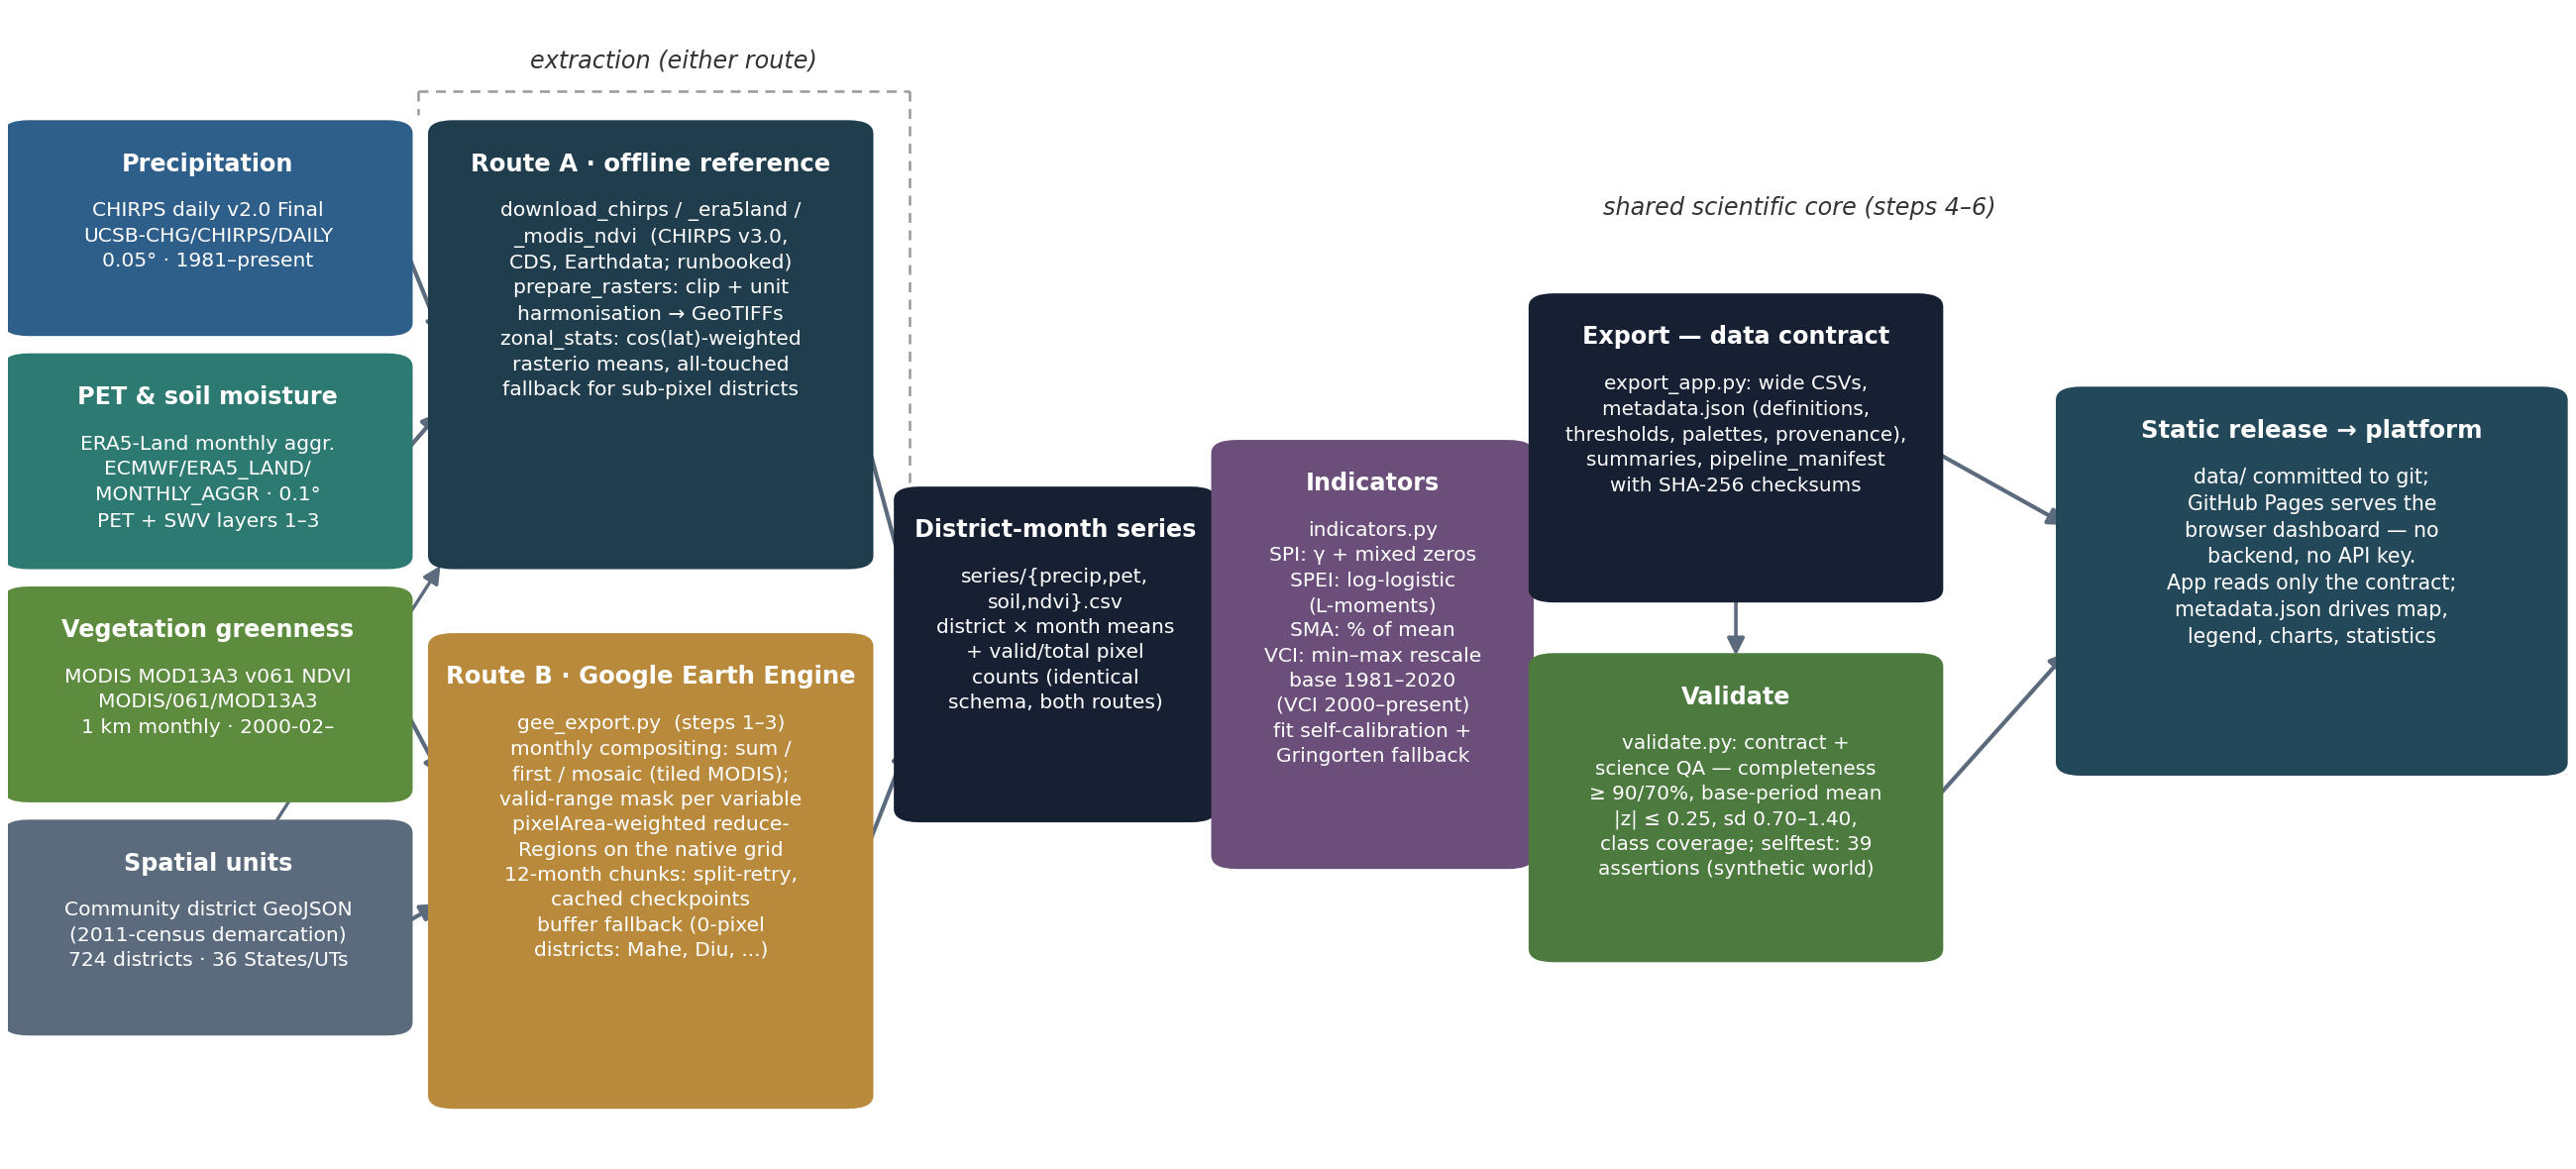
\includegraphics[width=\textwidth]{fig1_pipeline.png}
\caption{Data production chain of the Drought Intelligence Explorer (methodology version \texttt{research-gee-1.0.2}). Public sources are extracted through either of two interchangeable routes, an offline reference implementation (direct downloads, local rasterisation and zonal statistics) or Google Earth Engine server-side extraction, and converge on an identical district-month series schema. A shared scientific core computes the indicators, releases the versioned data contract and validates it. The two routes share code and schema; they use different source product versions for precipitation (v3.0 offline, v2.0 on Earth Engine), so extracted values are expected to agree closely but are not guaranteed identical. Every arrow is a scripted, re-runnable step; the module names and quality gates are printed in each box.}
\label{fig:pipeline}
\end{figure}

\begin{figure}[t]
\centering
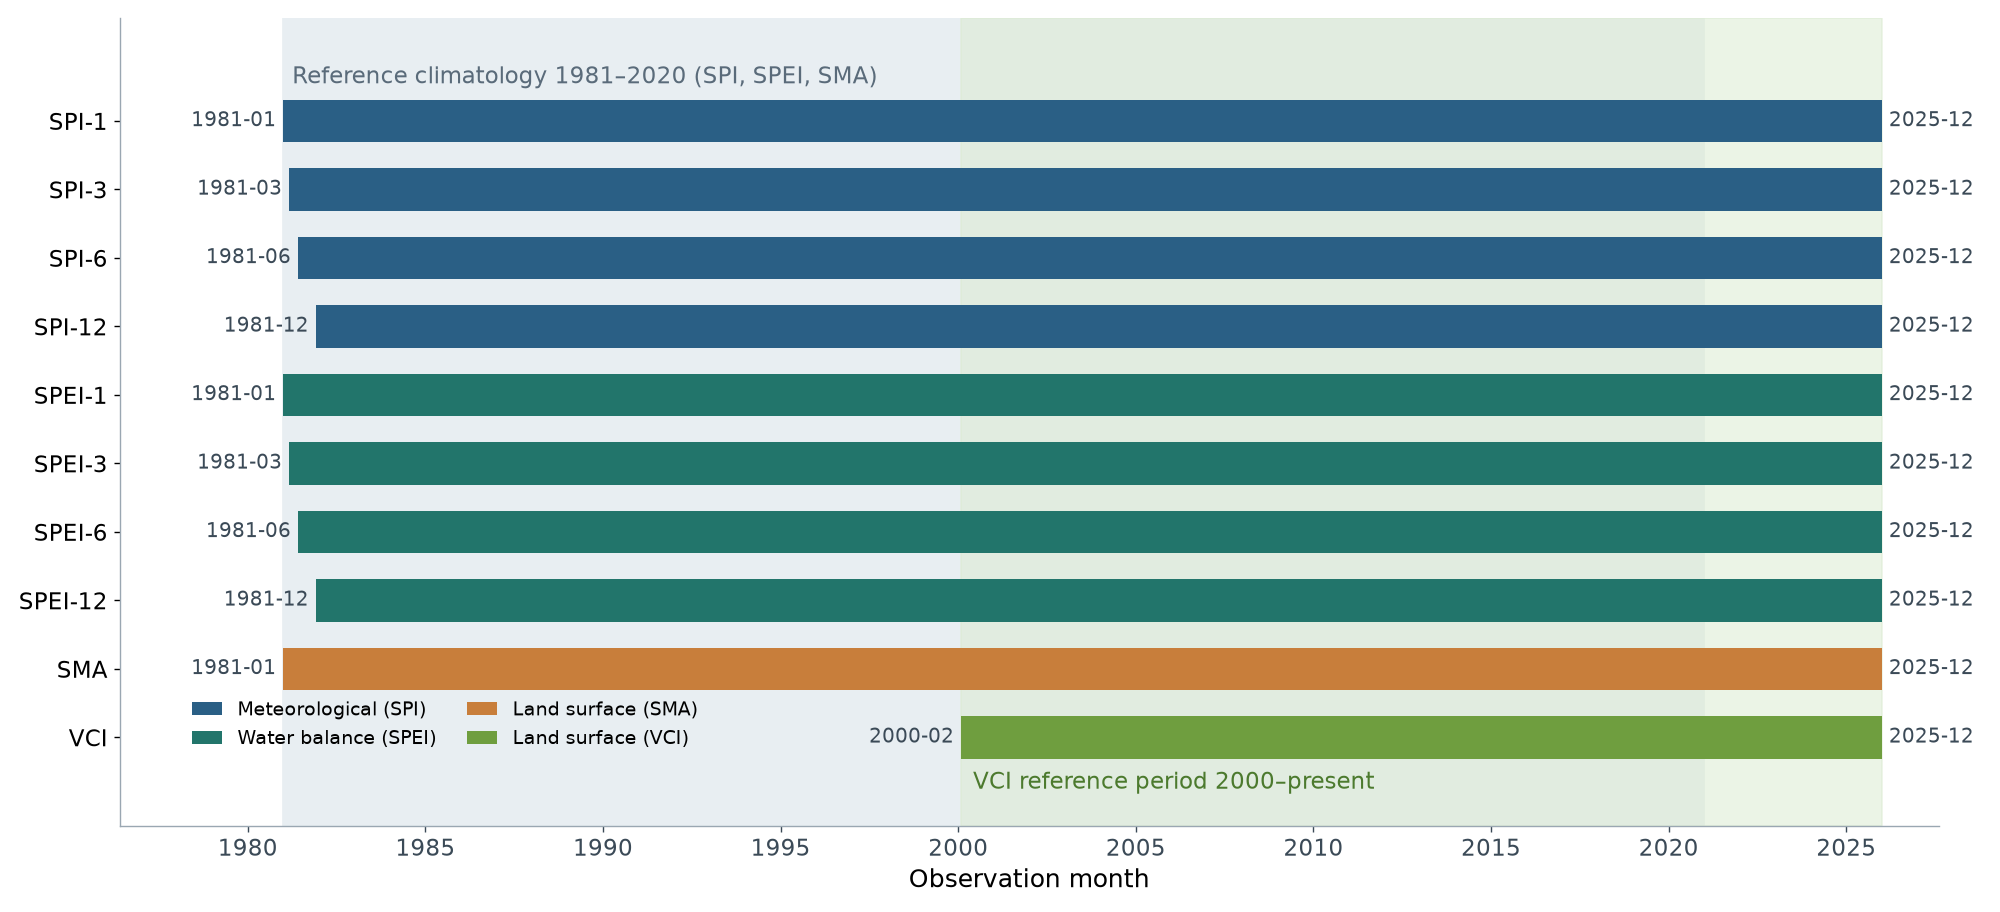
\includegraphics[width=\textwidth]{fig2_coverage.png}
\caption{Temporal coverage of the ten indicator matrices (1981--2025, monthly). Bars span each indicator's first to last available month; multi-month SPI and SPEI windows begin after their accumulation warm-up, and VCI begins with the MODIS NDVI record in February 2000. Shaded bands mark the standardization reference periods (1981--2020 for SPI, SPEI and SMA; 2000--present for VCI).}
\label{fig:coverage}
\end{figure}

A deliberate design principle throughout is verifiability. Sample sizes are reported on every chart, table and statistic; missing months are never imputed, interpolated or silently treated as normal, and appear as explicit gaps and no-data classes; parametric distribution fits are checked and fall back to a distribution-free transform rather than emitting unreliable values; the default methodology is always annotated and alternative event definitions are shown separately; uncertainty is quantified where defensible (bootstrap confidence intervals for correlations, rank-based intervals for trend slopes) and explicitly not claimed where it is not (empirical recurrence estimates); and correlation is never presented as causation. The sections that follow document the methods (Methods), the record layout (Data Records), the quality-control machinery (Technical Validation), how the platform is used in practice, including three worked examples with results read from the live deployment (Usage Notes), the reuse potential of the product, the scope of this version~1.0 and the planned future updates, and its limitations.

% =====================================================================
\section*{Methods}

\subsection*{Study area and spatial units}
The spatial unit is the administrative district. The build uses community-maintained district polygons with a 2011-era demarcation lineage (\texttt{github.com/udit-001/india-maps-data}, file \texttt{geojson/india.geojson}; retrieved 2026-11-02 for the build and 2026-11-10 for this paper). The source fabric distributes 760 polygon features. The boundary-preparation step (\texttt{prepare\_boundaries.py}) reconciles them to the 724 served districts by dropping 34 redundant state-level outline features (which carry no district name) and by removing two exact duplicate features: the source distributes the Lakshadweep and Chandigarh polygons twice with identical geometry. This leaves 726 $-$ 2 $=$ 724 districts across 36 States and Union Territories. The served fabric therefore contains the 724 unique district geometries of the source; the fabric includes district units created after the 2011 census, as supplied by the source, and is not tied to one official census vintage. The polygons are generalised for web delivery at approximately 100~m coordinate precision. Matching every served district against the unsimplified source geometry gives a median district-area error of 0.034\% and a 95th-percentile error of 0.15\%. Figure~\ref{fig:studyarea} shows the district fabric. The boundaries follow the depiction of the source dataset, carry no political endorsement and are not authoritative for legal boundary determination. The source repository currently states no explicit redistribution licence; the boundaries are therefore redistributed with full attribution and the disclaimer of the source, the licence status is being confirmed with the maintainers, and the boundary layer is separable from the archived dataset (see Data availability). District-level values are area aggregates of gridded fields, not point measurements, and the interface states this wherever indicators are described.

\begin{figure}[t]
\centering
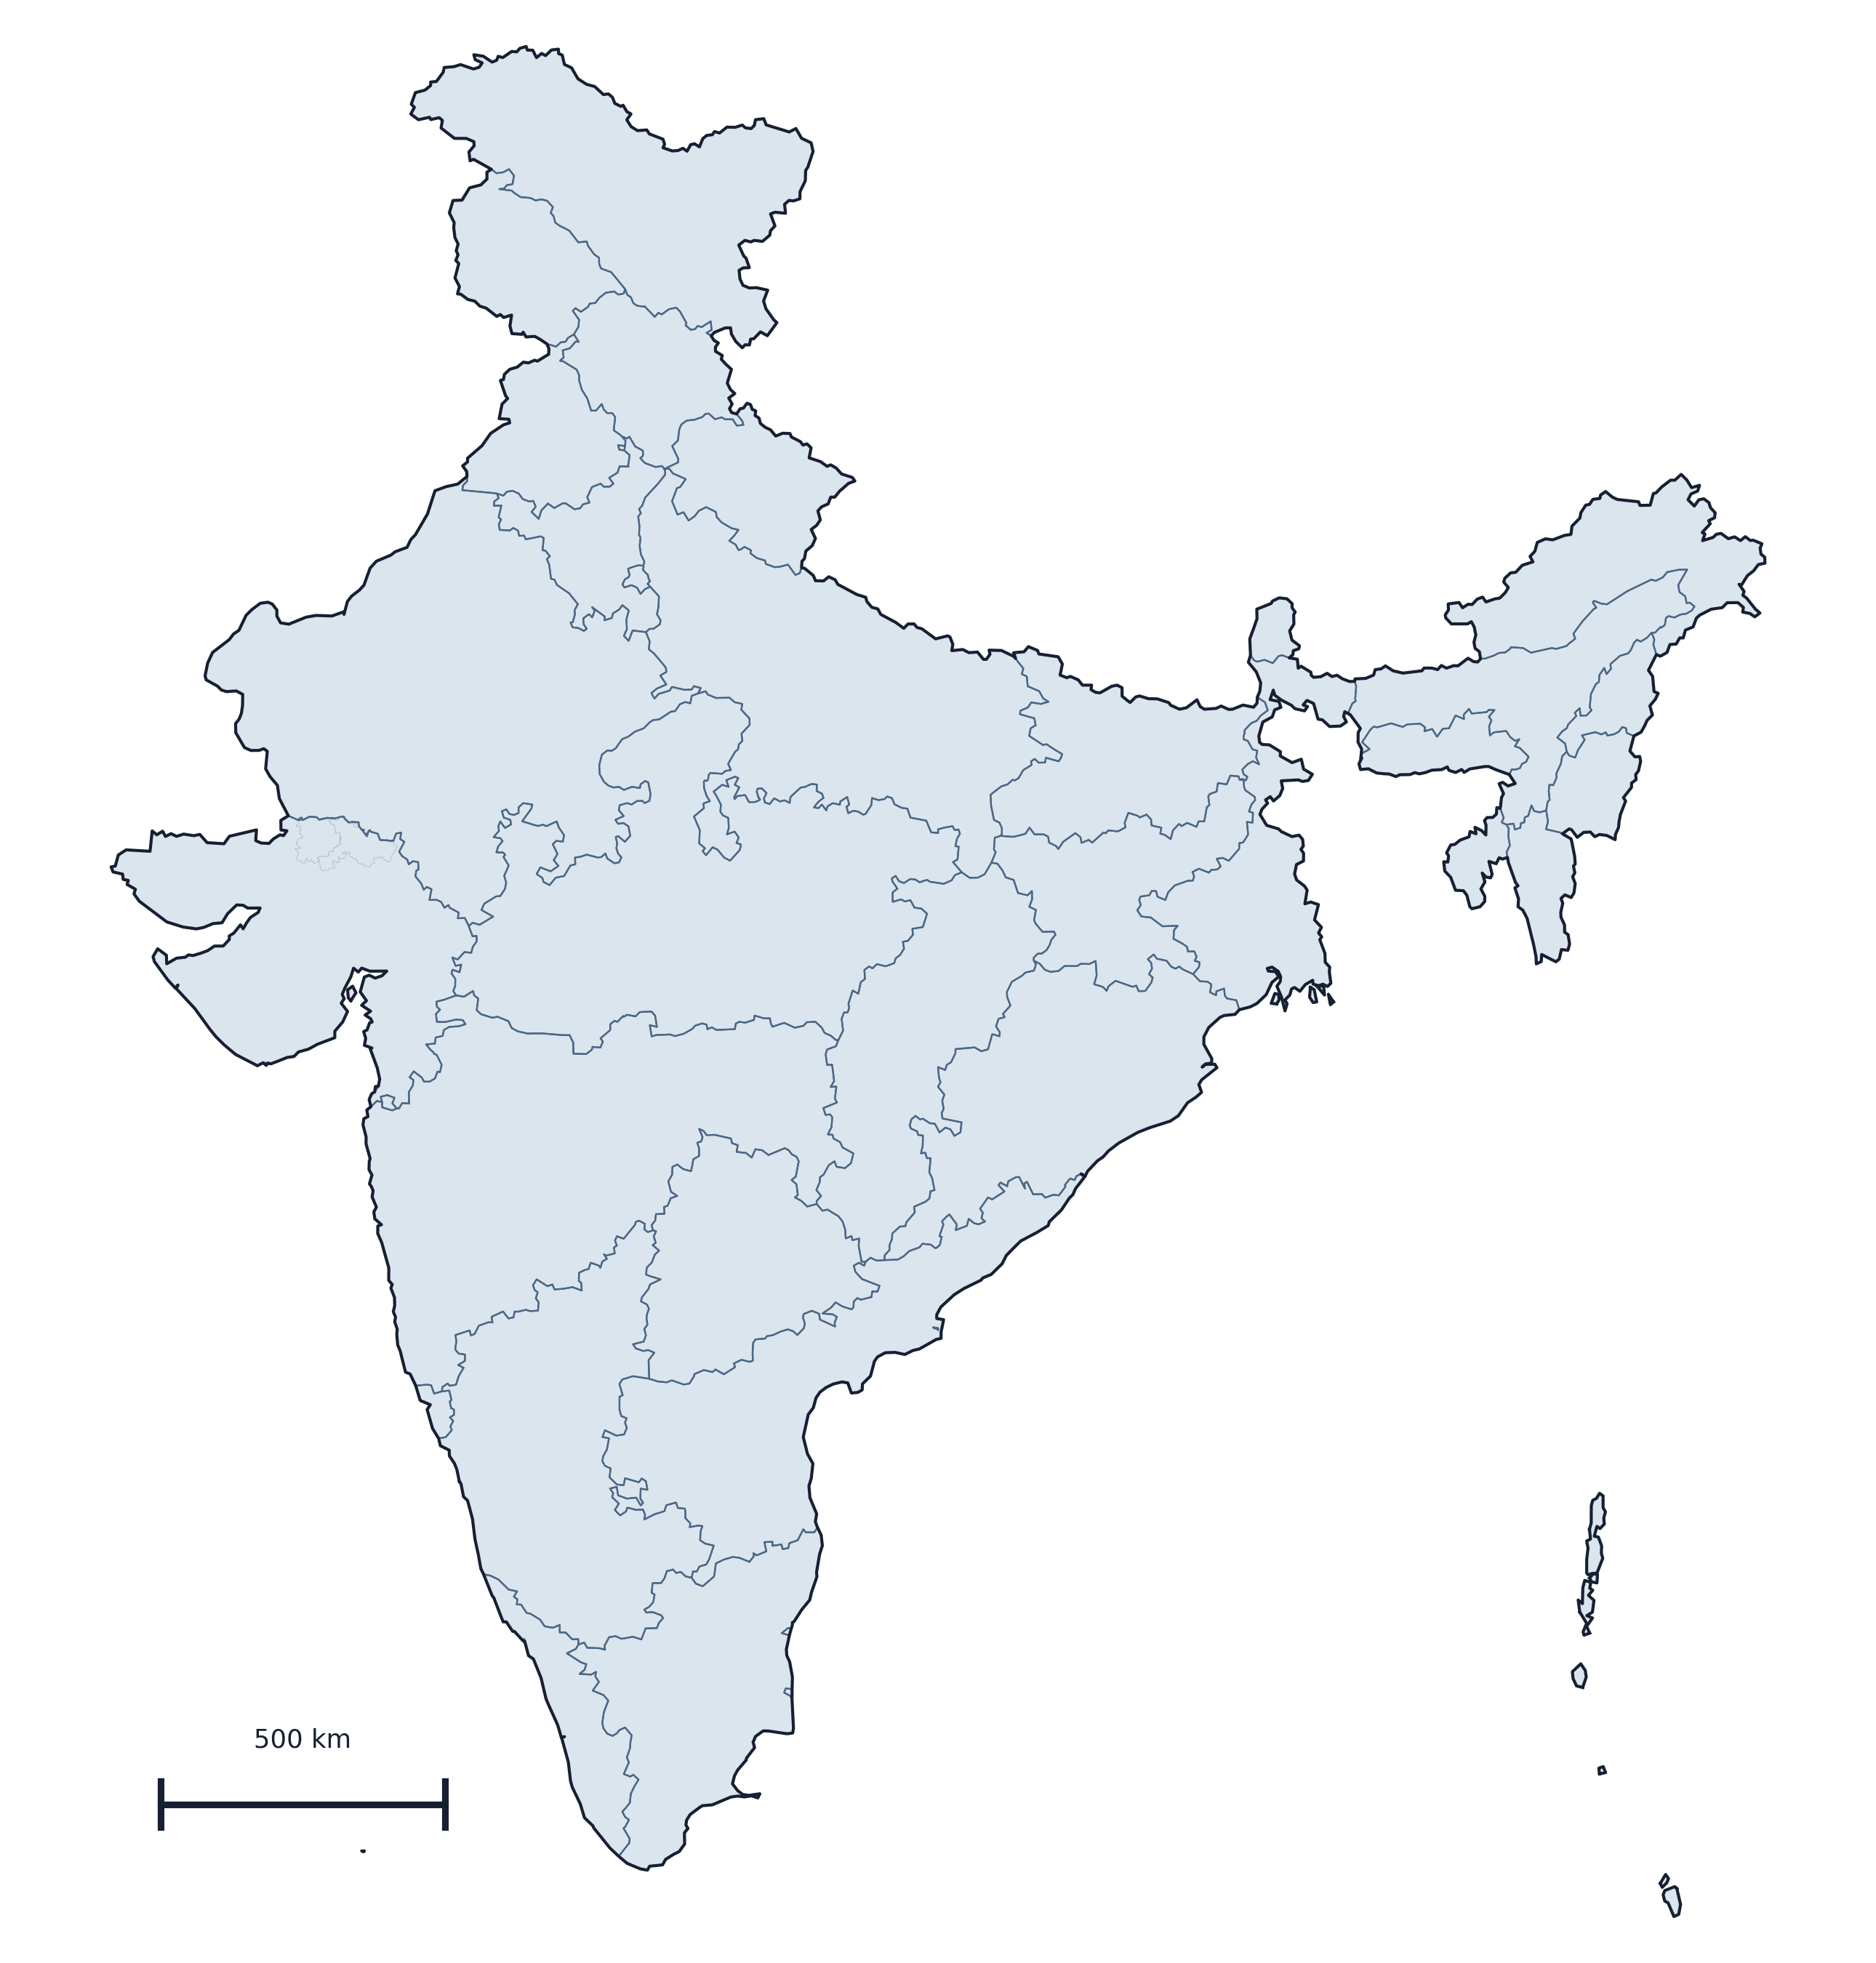
\includegraphics[width=0.82\textwidth]{fig3_study_area.png}
\caption{Study area and spatial units. The district polygons of the community source repository (\texttt{udit-001/india-maps-data}, 2011-era demarcation lineage), drawn in the Lambert Azimuthal Equal-Area projection used for all area statistics (\texttt{+proj=laea +lat\_0=22.5 +lon\_0=79.5}, WGS84); scale bar 500~km. The source distributes 760 polygon features; after dropping 34 state-level outline features and removing 2 exact duplicate features (Lakshadweep, Chandigarh), the platform serves 724 districts across 36 States and Union Territories at $\approx$100~m coordinate precision (median district-area error 0.034\%). Boundaries follow the source dataset's depiction, carry no political endorsement and are not authoritative for legal purposes. Geometry retrieved 2026-11-10 for this figure.}
\label{fig:studyarea}
\end{figure}

The choice of a stable district fabric is deliberate: a 45-year indicator series is only useful if the aggregation units remain stable over the whole archive, and the community fabric with a 2011-era demarcation lineage is the most complete openly available polygon set with consistent identifiers. Later district reorganisations would either fragment the record into units that did not exist for most of the period or force a spatio-temporal re-allocation of values that would itself introduce error; both are avoided by pinning the analysis units and documenting the vintage explicitly.

\subsection*{Source datasets}
Three public Earth-observation and reanalysis datasets feed the pipeline (Table~\ref{tab:sources}). Precipitation is the Climate Hazards Group InfraRed Precipitation with Stations (CHIRPS) daily product\citep{Funk2015}. The Earth Engine route, which produced the build documented here, reads the v2.0 Final collection (\texttt{UCSB-CHG/CHIRPS/DAILY}, band \texttt{precipitation}, mm per day) and sums it to monthly totals. The offline route instead downloads the CHIRPS v3.0 monthly global GeoTIFFs directly from the Climate Hazards Group server. The two routes therefore use different precipitation product versions; they share all downstream code and the identical schema, and their values are expected to agree closely, but they are not guaranteed identical and should not be mixed within one series. Potential evaporation (PET) and root-zone soil moisture come from the ERA5-Land monthly aggregated product\citep{MunozSabater2021} (collection \texttt{ECMWF/ERA5\_LAND/MONTHLY\_AGGR}, 0.1$^\circ$ grid). PET uses the \texttt{potential\_evaporation\_sum} band, an accumulated depth in metres per month that ECMWF reports as negative for upward (evaporative) flux; the pipeline takes its absolute value and converts it to millimetres per month. This is the reanalysis model's potential evaporation, not a FAO-56 Penman--Monteith reference evapotranspiration, and the two quantities differ by definition (see Limitations). Soil moisture uses the three \texttt{volumetric\_soil\_water\_layer} bands (m$^3$~m$^{-3}$), converted to percent volumetric, which together span 0--100~cm. ERA5-Land is the land-focused rebinding of the ERA5 reanalysis\citep{Hersbach2020}. Vegetation greenness uses the MODIS/Terra MOD13A3 v061 monthly NDVI product at 1~km\citep{Didan2015} (collection \texttt{MODIS/061/MOD13A3}, band \texttt{NDVI}, scale factor 0.0001). All three sources are public; CHIRPS is in the public domain, ERA5-Land is distributed under the Copernicus licence with attribution, and MOD13A3 is NASA open data. The pipeline also documents Indian Meteorological Department gridded rainfall and temperature products\citep{Pai2014,Srivastava2009} as alternative national inputs for an operational deployment.

\begin{table}[t]
\caption{Source datasets used by the research build, their access routes and periods used.}
\label{tab:sources}
\small
\begin{tabularx}{\textwidth}{@{}p{0.16\textwidth}p{0.20\textwidth}p{0.28\textwidth}p{0.12\textwidth}X@{}}
\toprule
Role & Dataset & Access route (Google Earth Engine collection) & Period used & Notes \\
\midrule
Precipitation (SPI, SPEI) & CHIRPS daily v2.0 Final & \texttt{UCSB-CHG/CHIRPS/DAILY}; offline route targets CHIRPS v3.0 & 1981--2025 & 0.05$^\circ$ grid; public domain \\
PET and soil moisture (SPEI, SMA) & ERA5-Land monthly aggregates & \texttt{ECMWF/ERA5\_LAND/MONTHLY\_AGGR} & 1981--2025 & 0.1$^\circ$; potential evaporation + volumetric soil water layers 1--3 (0--100~cm); Copernicus licence \\
Vegetation greenness (VCI) & MODIS/Terra MOD13A3 v061 NDVI & \texttt{MODIS/061/MOD13A3} & 2000-02--2025-12 & 1~km monthly; NASA open data \\
Spatial units & Community India district boundaries (2011-era demarcation) & \texttt{github.com/udit-001/india-maps-data}; processed by \texttt{prepare\_boundaries.py} & static & 724 districts, 36 States/UTs; generalised $\approx$100~m; median area error 0.034\% \\
\bottomrule
\end{tabularx}
\end{table}

\subsection*{Data pipeline architecture and extraction}
The production system is a six-stage pipeline (\texttt{data\_pipeline/}) with two interchangeable extraction routes that converge on an identical intermediate schema (Figure~\ref{fig:pipeline}). Route~A is an offline reference implementation: \texttt{download\_chirps.py}, \texttt{download\_era5land.py} and \texttt{download\_modis\_ndvi.py} fetch CHIRPS v3.0 monthly GeoTIFFs, ERA5-Land monthly means (Copernicus CDS) and MOD13A3 sinusoidal tiles (NASA Earthdata); \texttt{prepare\_rasters.py} clips each month to the national bounding box, harmonises units and applies physical valid-range guards; and \texttt{zonal\_stats.py} computes district means with pixel weights proportional to $\cos(\mathrm{latitude})$, with an all-touched rasterisation fallback for districts smaller than one pixel. Route~B, the route used for the build documented here, replaces the first three stages with a single server-side extraction through Google Earth Engine\citep{Gorelick2017}: \texttt{python run.py gee --project <project> --end 2025-12}. Steps 4--6 are shared by both routes. Sharing code and schema makes results transferable between routes, but it does not make the extracted values identical, because the routes read different precipitation product versions (v3.0 offline, v2.0 on Earth Engine); the pipeline documentation states this and warns against mixing series from the two routes in one analysis.

The Earth Engine route performs four operations per variable and month. First, monthly compositing in the source's native grid. CHIRPS daily accumulations are summed over the calendar month. ERA5-Land PET is read from the monthly aggregate, sign-corrected (the ECMWF convention records upward fluxes as negative) and converted from metres to millimetres. The three ERA5-Land soil-water layers (0--7, 7--28 and 28--100~cm) are averaged with equal weight per layer into a single 0--100~cm root-zone value in percent volumetric. This equal weighting is a documented simplification: the layers are unevenly thick, so the shallow layer contributes disproportionately. The depth-weighted alternative $\mathrm{SM}_{0\text{--}100}=(7\,\mathrm{SM}_1+21\,\mathrm{SM}_2+72\,\mathrm{SM}_3)/100$ is preferable in principle and is available as a pipeline modification; the released build keeps the equal-weight form because the indicator is a percent departure from climatology, whose sign and timing, and therefore its drought classification, are far less sensitive to the weighting than its amplitude. A quantitative sensitivity analysis of the two weightings is listed in the roadmap (Table~\ref{tab:roadmap}). The tiled MOD13A3 granules covering India are mosaicked into a single monthly image before the NDVI scale factor (0.0001) is applied; taking the first granule instead of mosaicking would mask most of the country to no-data. Every composite is masked to a physical valid range per variable (precipitation 0--4{,}000~mm/month, PET 0--1{,}500~mm/month, soil water 0--60\%, NDVI $-0.2$--1.0) before aggregation.

Second, area-weighted district aggregation. For each month a four-band stack is built (value $\times$ pixel area, valid pixel area, valid pixel count and total pixel count) and reduced over the 724 district polygons with \texttt{ee.Image.pixelArea()} as the area weight. Using \texttt{pixelArea()} rather than hand-computed $\cos(\mathrm{latitude})$ weights makes the identical code correct on the geographic CHIRPS and ERA5-Land grids and on the equal-area sinusoidal MODIS grid. The reduction runs on each source's native projection and affine transform, which are read explicitly from the first raw image: derived images lose projection metadata, and without explicit pinning Earth Engine would silently fall back to a 1$^\circ$ default grid and make total pixel counts meaningless.

Third, robustness engineering appropriate to a 540-month batch extraction. Requests are chunked at 12 months per \texttt{reduceRegions} call with a \texttt{tileScale} of 4 (raised to 8 if Earth Engine reports memory errors); a failing chunk is recursively split in half and retried; completed chunks are cached as CSV checkpoints and only reused when their month coverage matches exactly. Districts whose only overlapping pixels are masked receive a buffer fallback: the polygon is expanded by a per-variable buffer and the reduction is repeated over the buffered geometry. The buffer distance is matched to each source's grid spacing (6~km for precipitation at 0.05$^\circ$, 16~km for PET and soil water at 0.1$^\circ$, 2~km for NDVI at $\approx$1~km) and is applied only to districts whose total pixel count is zero, so no normal district aggregate is ever modified. The buffered districts are counted and printed in the build log. A buffered value mixes the district's own land (if any) with pixels from outside the boundary, so it is a nearest-neighbour estimate rather than a true district mean; this matters only for a few very small island units (Mahe, Lakshadweep, Diu) whose share of the national surface is negligible, and even the 16~km buffer finds no valid ERA5-Land pixel for Lakshadweep, which stays honestly missing (Data Records). Because \texttt{reduceRegions} weights pixels by the fraction of their area inside each polygon, the returned pixel counts are fractional and are rounded to integers, with non-null means never carrying a zero count.

Fourth, provenance capture. The run writes a JSON metadata block recording the project, window, chunking parameters, native grids, dataset identifiers and the months actually available in each collection; months that the catalogue does not yet contain are skipped and reported rather than silently filling the series with gaps.

A methodological decision worth stating explicitly is that the indices are \emph{not} computed inside Earth Engine. SPI and SPEI require per-district, per-calendar-month distribution fits over the 40-year base period and an inverse-normal transform, statistical machinery that Earth Engine's reducer library does not provide, while the fits themselves are small, fast client-side operations. Keeping the statistics in a small, audited Python module (\texttt{indicators.py}) keeps them testable offline, versionable and independent of the extraction vendor: the offline route and the Earth Engine route feed the identical schema, and the indicator, export and validation steps are byte-for-byte shared. The pipeline is verified end-to-end offline by \texttt{selftest.py}, which builds a synthetic data world with an injected drought, NDVI gaps and a missing soil month, and asserts 82 invariants across the compute chain, the exported contract and the validation gates (seed-deterministic; the validation stage alone contributes 55 contract and science checks). Table~\ref{tab:stages} lists the stages, their commands and their guarantees.

\begin{table}[t]
\caption{Pipeline stages, entry points and guarantees. Stages 1--3 exist in two interchangeable implementations (offline and Google Earth Engine) that write the identical intermediate schema; stages 4--6 are shared.}
\label{tab:stages}
\small
\begin{tabularx}{\textwidth}{@{}p{0.055\textwidth}p{0.235\textwidth}p{0.30\textwidth}X@{}}
\toprule
Stage & Module (command) & Function & Output / guarantee \\
\midrule
0 & \texttt{selftest.py} (\texttt{python selftest.py}) & Offline end-to-end test on a synthetic world with an injected drought & 82 assertions must pass before any release \\
1a & \texttt{download\_chirps.py}, \texttt{download\_era5land.py}, \texttt{download\_modis\_ndvi.py} (\texttt{run.py update}) & Direct downloads: CHIRPS v3.0 (no auth), ERA5-Land (CDS), MOD13A3 (Earthdata) & Monthly raw archive; idempotent, retrying fetch of missing months \\
2a & \texttt{prepare\_rasters.py} & Clip to national bounding box, unit harmonisation, valid-range guards & Monthly GeoTIFFs in physical units \\
3a & \texttt{zonal\_stats.py} & $\cos(\mathrm{latitude})$-weighted district means + pixel counts; all-touched fallback for sub-pixel districts & \texttt{series/\{precip,pet,soil,ndvi\}.csv} \\
1b--3b & \texttt{gee\_export.py} (\texttt{run.py gee}) & Server-side monthly compositing, valid-range masking, \texttt{pixelArea()}-weighted \texttt{reduceRegions} on native grids; 12-month chunks, split-retry, cached checkpoints, buffer fallback & Same \texttt{series/*.csv} schema; run metadata with grids and month availability \\
4 & \texttt{indicators.py} (\texttt{run.py indicators}) & SPI, SPEI, SMA, VCI with per-fit calibration checks and empirical fallback & \texttt{indicators/*.csv} + fit report (\texttt{\_report.json}) \\
5 & \texttt{export\_app.py} (\texttt{run.py export}) & Write the application data contract & Wide CSVs, \texttt{metadata.json}, summaries, \texttt{pipeline\_manifest.json} with SHA-256 checksums \\
6 & \texttt{validate.py} (\texttt{run.py validate}) & Contract checks + scientific QA gates & Non-zero exit code blocks release \\
\bottomrule
\end{tabularx}
\end{table}

\subsection*{Indicator computation}
Ten indicators are computed per district and calendar month (Table~\ref{tab:indicators}). SPI is computed from accumulated precipitation at 1-, 3-, 6- and 12-month windows\citep{McKee1993}: for each district, calendar month and window, a two-parameter gamma distribution is fitted by maximum likelihood to the positive accumulation totals of the reference period, a mixed distribution $H(x) = q + (1-q)\,G(x)$ handles zero-rain months ($q$ the base-period probability of a dry month), and the observed accumulation is mapped through the fitted non-exceedance probability to the standard normal deviate. The gamma family is the conventional and, in large-sample evaluations, at-or-near best-behaved choice across climates\citep{Stagge2015}; the mixed-distribution treatment of zeros is required in semi-arid districts where dry calendar months occur, and months whose rolling window is incomplete remain missing rather than being mapped through the CDF floor, which would otherwise encode warm-up months as record droughts.

SPEI applies the same logic to the water balance (precipitation minus PET): a three-parameter log-logistic distribution is fitted with the probability-weighted-moment (L-moment) closed-form estimator recommended for SPEI\citep{VicenteSerrano2010,Begueria2014}, with the L-moments computed by their unbiased probability-weighted-moment estimators\citep{Hosking1990}. Maximum likelihood is deliberately not used for SPEI. In our simulation experiments, at the operational sample size of 30--40 base years the maximum-likelihood fit drives the log-logistic location parameter onto the sample minimum with a vanishing scale, biasing every transformed value wet, whereas the L-moment estimator remains calibrated. This small-sample MLE critique follows Beguer\'{\i}a et al.~\citeyearpar{Begueria2014}. The quantified figure quoted in this paper comes from a specific simulation, not from a general theorem: 300 synthetic replications of log-logistic samples with parameters typical of Indian district-month water-balance series, at $n=40$, gave a mean transformed base value of $+0.79$ standard deviations under maximum likelihood against $+0.01$ under L-moments. The simulation script is released with the pipeline so that the design, the parameters and the sample-size sensitivity can be inspected and re-run (see Code availability). Every parametric fit is additionally checked against its own base sample: the transformed base values must have a mean within $\pm0.2$ of zero and a standard deviation between 0.75 and 1.3. Where a fit is unstable, or the sample skew is incompatible with the log-logistic family, the implementation falls back to a distribution-free Gringorten plotting-position transform\citep{Gringorten1963}. The fallback replaces the parametric fit for the \emph{entire} district-calendar-month series (never for selected observations), assigns tied observations their average (mid) rank, and maps the rank $i$ of $n$ ordered values to the probability $p_i=(i-0.44)/(n+0.12)$ before the inverse-normal transform. Zero-inflated series are handled by the same rank rule: an all-zero base month maps every year to $z\approx0$ (``identical to climatology'') instead of the spurious ``extremely wet'' artifact that a naive interpolation over duplicated values produces. The share of district-months using the parametric fit versus the fallback is written to the per-run fit report (\texttt{\_report.json}), so it is auditable for every build; no unreliable standardized value is ever emitted.

The SMA expresses root-zone (0--100~cm) soil moisture as the departure of each month from the same calendar month's base-period climatology, in per cent of the climatological mean:
\[
\mathrm{SMA}_{i,t}=100\times\frac{\mathrm{SM}_{i,t}-\overline{\mathrm{SM}}_{i,\,m(t)}}{\overline{\mathrm{SM}}_{i,\,m(t)}},
\]
where $\overline{\mathrm{SM}}_{i,\,m}$ is the 1981--2020 mean of the calendar month $m(t)$ for district $i$. Negative values are deficits, and the class thresholds ($-5/-15/-30/-50$\%) are defined against this statistic. The per-cent-of-mean form was selected over the z-score form because it preserves the operational interpretability of ``drier than the seasonal normal by X\%'' for practitioner audiences; a z-score variant exists as a documented configuration switch (with the class table remapped accordingly). Because SMA is a percentage departure from a positive climatological mean, it is a bounded-ratio indicator, not a standardized z-score, and it is treated as such throughout (classification, event thresholds and aggregation).

The VCI rescales NDVI between its historical minimum and maximum\citep{Kogan1995}:
\[
\mathrm{VCI}_{i,t}=100\times\frac{\mathrm{NDVI}_{i,t}-\mathrm{NDVI}^{\min}_{i,\,m(t)}}{\mathrm{NDVI}^{\max}_{i,\,m(t)}-\mathrm{NDVI}^{\min}_{i,\,m(t)}},
\]
where $\mathrm{NDVI}^{\min}_{i,\,m}$ and $\mathrm{NDVI}^{\max}_{i,\,m}$ are the minimum and maximum of the \emph{district-month} NDVI series for calendar month $m$ over the base period, and values are clipped to $[0,100]$. Two implementation facts matter for interpretation. First, the spatial order of operations: NDVI is aggregated to districts first (area-weighted pixel mean), and the VCI is computed from the aggregated district series, so VCI is a rescaling of district-mean greenness, not an area-weighted mean of pixel-level VCI values; the two constructions are not equivalent, and this one matches the operational practice of computing index values per reporting unit. Second, the base period is 2000 to the release date rather than a fixed window, because the MODIS record is short and its early years are the least reliable; the minima and maxima are therefore frozen within each dataset release, and a future release that extends the record can shift them, which changes VCI values for all years. Each release is a self-consistent version, the change is documented in the release notes, and a fixed 2001--2020 VCI baseline is listed in the roadmap (Table~\ref{tab:roadmap}).

Standardization always uses per-calendar-month distributions over a fixed reference period, which is what makes values comparable across districts and years. The reference period is 1981--2020, a fixed 40-year window, for SPI, SPEI and SMA; VCI uses 2000 to the release date, which is limited by the start of the MODIS record. A 40-year baseline was chosen over the WMO 30-year normal\citep{WMOLincoln2009} for statistical rather than climatological reasons: the standardization fits one distribution per district and calendar month, so the sample for a January fit is 40 values, not 40 years times 12 months, and 30 values per fit sit too close to the minimum sample for a stable three-parameter fit. The longer window trades a little climatological currency for much more robust fitting, and it is held constant across the released archive so that values remain comparable across the whole record and across dataset versions. Values after December 2020 are therefore out-of-sample standardizations: they are mapped through distribution parameters fitted on 1981--2020, which is the intended behaviour of a fixed climatology but should be kept in mind when reading the most recent years. A hard floor of 20 base years per district-month fit prevents standardization on climatically meaningless samples. Multi-month windows begin only once the first rolling accumulation is complete, so SPI-3, SPI-6 and SPI-12 start in March 1981, June 1981 and December 1981 respectively (Figure~\ref{fig:coverage}). SPI and SPEI are classified with the conventional nine-category scheme (Table~\ref{tab:classes}): the class edges are inclusive on the dry side, so a value of $-2.00$ is extreme drought. SMA and VCI are bounded percentages and deliberately do not reuse the z-score thresholds, which would be invalid for them; their class edges ($-5/-15/-30/-50$\% for SMA) are operational conventions of this build rather than internationally standardised cut-offs. They are defined once in the metadata file, applied consistently everywhere, and can be reconfigured there if a deployment adopts a different convention. All thresholds, units, palettes and descriptions are stored in a single metadata file that drives the map, the legend, the charts and the statistics, so the classification shown to the user is by construction the classification used in every computation.

\begin{table}[t]
\caption{The ten indicators: families, definitions, units and availability.}
\label{tab:indicators}
\small
\begin{tabularx}{\textwidth}{@{}l l X l l@{}}
\toprule
Indicator & Family & What it standardises & Units & Availability \\
\midrule
SPI-1 & Meteorological & Accumulated precipitation, 1-month window & z-score & 1981-01--2025-12 \\
SPI-3 & Meteorological & Accumulated precipitation, 3-month window & z-score & 1981-03--2025-12 \\
SPI-6 & Meteorological & Accumulated precipitation, 6-month window & z-score & 1981-06--2025-12 \\
SPI-12 & Meteorological & Accumulated precipitation, 12-month window & z-score & 1981-12--2025-12 \\
SPEI-1 & Water balance & Precipitation minus PET, 1-month window & z-score & 1981-01--2025-12 \\
SPEI-3 & Water balance & Precipitation minus PET, 3-month window & z-score & 1981-03--2025-12 \\
SPEI-6 & Water balance & Precipitation minus PET, 6-month window & z-score & 1981-06--2025-12 \\
SPEI-12 & Water balance & Precipitation minus PET, 12-month window & z-score & 1981-12--2025-12 \\
SMA & Land surface & Root-zone (0--100~cm) soil moisture departure from seasonal climatology & \% & 1981-01--2025-12 \\
VCI & Land surface & NDVI rescaled between historical stress and optimum & \% & 2000-02--2025-12 \\
\bottomrule
\end{tabularx}
\end{table}

\begin{table}[t]
\caption{Severity classification. SPI and SPEI use the conventional nine-category z-score scheme; SMA and VCI use their own bounded-percentage conventions.}
\label{tab:classes}
\small
\begin{tabularx}{\textwidth}{@{}l l X@{}}
\toprule
SPI / SPEI class & Range (z-score) & SMA class (range, \%) $\cdot$ VCI class (range, \%) \\
\midrule
Extreme drought & $\le -2.00$ & Extreme anomaly ($\le -50$) $\cdot$ Extreme vegetation stress (0--10) \\
Severe drought & $-2.00$ to $-1.50$ & Severe anomaly ($-50$ to $-30$) $\cdot$ Severe vegetation stress (10--20) \\
Moderate drought & $-1.50$ to $-1.00$ & Moderate anomaly ($-30$ to $-15$) $\cdot$ Moderate vegetation stress (20--30) \\
Mild drought & $-1.00$ to $-0.50$ & Mild anomaly ($-15$ to $-5$) $\cdot$ Mild vegetation stress (30--40) \\
Near normal & $-0.50$ to $0.50$ & Near normal ($-5$ to $+5$) $\cdot$ Normal vegetation condition (40--60) \\
Mildly wet & $0.50$ to $1.00$ & Wet anomaly ($\ge +5$) $\cdot$ Favourable conditions (60--100) \\
Moderately wet & $1.00$ to $1.50$ & not used \\
Severely wet & $1.50$ to $2.00$ & not used \\
Extremely wet & $\ge 2.00$ & not used \\
\bottomrule
\end{tabularx}
\end{table}

\subsection*{Design choices and their justification}
Table~\ref{tab:choices} consolidates the methodological decisions that most affect results, the principal alternative considered for each, and the justification, by citation where the literature settles the question and by explicit scientific or engineering logic where it does not. Table~\ref{tab:engchoices} lists the data-engineering and reproducibility choices separately, so that the statistical decisions are not buried among the plumbing. The intent is that a reviewer or re-user can challenge any individual decision without re-deriving the whole chain.

\begin{table}[t]
\caption{Methodological choices, the alternatives considered and their justification (citation or logic).}
\label{tab:choices}
\footnotesize
\begin{tabularx}{\textwidth}{@{}p{0.17\textwidth}p{0.20\textwidth}p{0.20\textwidth}X@{}}
\toprule
Decision & Selected approach & Principal alternative & Justification \\
\midrule
Which drought facets to cover & SPI, SPEI, SMA, VCI at four accumulation windows & One composite index & Meteorological, agricultural and land-surface drought respond on different timescales\citep{WilhiteGlantz1985,MishraSingh2010}; composite indices require weighting judgements that are hard to defend universally\citep{HaoSingh2015}. Families are kept separate and interpretable\citep{SvobodaFuchs2016}. \\
SPI distribution & Two-parameter gamma + mixed-distribution zeros & Generalised extreme value or Pearson III & The NCAR \texttt{climate\_indices} convention\citep{McKee1993}; gamma performs at or near best across climatic regimes in large-sample evaluations\citep{Stagge2015}. \\
SPEI parameter fitting & Three-parameter log-logistic fitted by L-moments & Maximum likelihood & MLE of the log-logistic location is degenerate at $n\approx30$--40 (wet bias $\approx+0.8$~z in our simulations); L-moments are unbiased and recover known parameters almost exactly\citep{Begueria2014,Hosking1990}. \\
Failed or degenerate fits & Tie-aware Gringorten empirical transform & Clip to the CDF floor and publish & Standardized values should never be published from an uncalibrated fit\citep{Stagge2015}; the average-rank Gringorten transform\citep{Gringorten1963} handles ties (e.g.\ all-zero months) without wet-side artifacts. \\
Reference period & Fixed 40-year 1981--2020 (SPI, SPEI, SMA); 2000--release (VCI) & Rolling or trailing climatology; 30-year WMO normal & 40 values per district-month fit is the practical minimum for stable three-parameter fits; a fixed window keeps values comparable across the archive and across dataset versions\citep{WMOLincoln2009,SvobodaFuchs2016}. \\
PET source & ERA5-Land \texttt{potential\_evaporation\_sum} (sign-corrected, mm/month) & Temperature-based (Hargreaves) from interpolated stations & Physically based and mutually consistent with the soil-moisture fields of the same reanalysis\citep{MunozSabater2021}; reanalysis PET, not FAO-56 reference ET (see Limitations). \\
Root-zone soil water & Equal-weight mean of the three ERA5-Land layers (v1.0.0) & Thickness-weighted $(7,21,72)$~cm mean & Equal weighting is a documented simplification; the anomaly's sign and timing are far less sensitive to weighting than its amplitude; sensitivity analysis on the roadmap. \\
MODIS quality screening & Physical valid-range guard only (v1.0.0) & \texttt{DetailedQA}/pixel-reliability screening & Monthly compositing, area aggregation and min/max baselines mitigate contamination; per-pixel QA screening is planned (see Source datasets and Limitations). \\
Trend machinery & Mann--Kendall + Sen's slope + Hamed--Rao correction & Ordinary least squares only & Monthly indices are serially autocorrelated, inflating naive significance; rank-based tests are robust to non-normality\citep{Mann1945,Sen1968,HamedRao1998}. \\
Lag uncertainty & Moving-block bootstrap (1{,}000 resamples, fixed seed) & Independent bootstrap & Block resampling preserves the serial dependence of monthly series\citep{Kunsch1989}. \\
\bottomrule
\end{tabularx}
\end{table}

\begin{table}[t]
\caption{Data-engineering and reproducibility choices, the alternatives considered and their justification.}
\label{tab:engchoices}
\footnotesize
\begin{tabularx}{\textwidth}{@{}p{0.17\textwidth}p{0.20\textwidth}p{0.20\textwidth}X@{}}
\toprule
Decision & Selected approach & Principal alternative & Justification \\
\midrule
District aggregation & \texttt{pixelArea()}-weighted areal mean with valid/total pixel counts & Unweighted pixel mean & Area-proportional weighting is correct on geographic and equal-area grids alike\citep{Gorelick2017}; pixel counts expose small-sample districts to the user. \\
Spatial units & 724 districts, 2011-era demarcation, generalised $\approx$100~m & Latest administrative fabric & Series consistency outweighs administrative currency: post-2011 units do not exist for most of the record, and re-allocating values across vintages would introduce error (logic; see Study area). \\
Sub-pixel districts & Per-variable buffer fallback, only when pixel count is zero & Leave missing & Nearest-neighbour estimate beats a hole for a few island units; buffer is grid-matched (6/16/16/2~km), logged, and flagged as a support change (see Pipeline). \\
Missing data & Never imputed; gaps, no-data classes, valid counts & Interpolation or carry-forward & Gaps carry information; imputation would fabricate drought classes and corrupt runs statistics (logic; policy in Methods). \\
Where indices are computed & Extraction in Earth Engine; statistics client-side & Compute indices in Earth Engine & Earth Engine has no gamma/log-logistic reducer; small audited Python modules are offline-testable (\texttt{selftest.py}) and vendor-independent (logic\citep{Gorelick2017}). \\
VCI aggregation order & District-mean NDVI first, then index rescaling & Pixel-level VCI, then area-weighting & Matches per-unit operational practice; the two constructions differ and the choice is stated explicitly (see Indicator computation). \\
\bottomrule
\end{tabularx}
\end{table}

\subsection*{Spatial aggregation and area statistics}
Regional summaries are area-weighted: the mean of an indicator over any region is the sum of district values weighted by district area, divided by the total valid area,
\[
\bar{x}_{R}=\sum_{i\in R} w_i\,x_i \Big/ \sum_{i\in R} w_i ,\qquad w_i=\frac{A_i}{\sum_{j\in R}A_j},
\]
and drought-affected area is the equal-area surface of districts in drought classes expressed in km$^2$ and as a share of the region. Areas are precomputed in a Lambert Azimuthal Equal-Area projection centred on India (\texttt{+proj=laea +lat\_0=22.5 +lon\_0=79.5}, WGS84 datum), never from degree-coordinate arithmetic, and are computed from the same generalised geometry that the map serves. The served national total is 3{,}266{,}386~km$^2$ against India's published area of 3{,}287{,}263~km$^{2}$, a shortfall of 20{,}877~km$^2$ or 0.64\%. Where does that shortfall come from? We measured it. The unsimplified source fabric, evaluated in the same projection, totals 3{,}266{,}465~km$^2$ for the 726 district features, or 3{,}266{,}382~km$^2$ for the 724 unique districts once the two exact duplicate features are removed. Generalisation therefore accounts for about 4~km$^2$, effectively nothing. The remaining 20{,}881~km$^2$ (0.63\%) is present in the community source fabric itself: it reflects the source's coastline generalisation, its treatment of disputed and ill-surveyed stretches, and its small-island coverage. The shortfall is thus a property of the boundary source, not of the pipeline's simplification, and it is stated rather than corrected because no single official district-level geometry exists for all of India in open form. The state-level statistics shipped as a cross-check file are computed with the same area-weighting rule, which was verified on the released build (see Technical Validation). Unweighted means are never used for regional summaries, and every aggregated statistic reports the number of valid districts ($n$) contributing to it.

\subsection*{Drought event identification}
Discrete drought events are identified by runs analysis on the continuous monthly series\citep{Yevjevich1967}. The truncation level $\tau$ is the upper bound of the moderate-drought class of the current indicator, that is $-1.00$ for SPI/SPEI, $-15$\% for SMA and 30\% for VCI, so event identification stays consistent with the classification legend for every indicator. A run qualifies as an event when it lasts at least three consecutive months; isolated one- or two-month excursions below the truncation level are not events. For each event the catalogue records onset, termination, duration, maximum intensity, cumulative severity and mean intensity, and recovery:
\[
\text{severity}=\sum_{t\in \text{event}} \max\!\left(0,\ \tau-x_t\right),\qquad
\text{mean intensity}=\frac{\text{severity}}{\text{duration}},
\]
so the same deficit-below-truncation definition, in the indicator's own units, applies to every family. Maximum intensity is the event's driest month: the minimum value for SPI, SPEI and SMA, and the lowest VCI (strongest vegetation stress) for VCI. Recovery is defined for the signed families (SPI, SPEI, SMA) as the number of months from the event's end to the first value at or above zero, a return to neutral conditions, which is stricter than merely exiting the drought class. For VCI, whose values are bounded between 0 and 100, a value of zero is the scale's floor rather than a neutral state, so the recovery-to-neutral statistic is not meaningful and is reported as unavailable for VCI events in this release; VCI recovery should be read either as the event end (return above the 30\% truncation) or, in a future release, as return to the normal-vegetation class (VCI $\ge$ 40), and the interface notes this. Events that touch the start or end of the record or of the analysis period are flagged as censored, because their true onset or termination may lie outside the observed window; censored events remain listed but are excluded from duration and severity rankings. Missing months break runs, with no interpolation or carry-forward. A first-class sensitivity panel re-runs the catalogue under alternative minimum durations (4, 6, 9 and 12 months) and truncation levels ($-0.50$, $-1.50$ and $-2.00$), always annotating the default definition and visually separating non-default results (Table~\ref{tab:events}).

\begin{table}[t]
\caption{Drought event definition and the sensitivity scenarios exposed by the platform.}
\label{tab:events}
\small
\begin{tabularx}{\textwidth}{@{}p{0.17\textwidth}p{0.34\textwidth}X@{}}
\toprule
Parameter & Default (documented methodology) & Alternative scenarios \\
\midrule
Truncation level & Upper bound of the moderate-drought class of the current indicator ($-1.00$ z-score; $-15$\% SMA; 30\% VCI) & $-0.50$, $-1.50$, $-2.00$ (z-score indicators); scenario runs re-compute the full catalogue \\
Minimum duration & 3 consecutive months & 4, 6, 9, 12 months \\
Severity & Sum of deficits below the truncation level over event months (indicator units) & Recomputed per scenario \\
Mean intensity & Severity $\div$ duration & Recomputed per scenario \\
Recovery & Months from event end to first value $\ge 0$ (SPI/SPEI/SMA); not applicable to VCI on its bounded scale & Undefined (blank) when the record ends first \\
Censoring & Events touching the record or period edge are flagged and excluded from rankings & Flag always reported \\
\bottomrule
\end{tabularx}
\end{table}

\subsection*{Trend analysis}
Two tiers of trend information are provided, clearly separated. Descriptive ordinary-least-squares trends are offered on the time-series chart only when at least 120 valid monthly observations exist, and are labelled as a simple diagnostic. Inferential trend testing uses the Mann--Kendall test\citep{Mann1945,Kendall1975} with tie-corrected variance, reported as the $S$ statistic, $Z$ and the two-sided $p$-value, together with Sen's slope\citep{Sen1968}, the median of pairwise slopes, and its rank-based 90\% confidence interval\citep{Gilbert1987}. Because monthly drought indices are serially autocorrelated, which inflates naive significance, the detrended series is tested for autocorrelation at lags 1--12 against the $1.96/\sqrt{n}$ white-noise bound; where significant autocorrelation is found, the Hamed--Rao variance correction\citep{HamedRao1998} is applied, the effective sample size is computed from the significant autocorrelations, and both corrected and uncorrected $Z$ values are reported with an explicit statement of which is in force. The default trend input is the annual regional-mean series: the twelve calendar months of each year are averaged into one annual value, with at least nine valid months required for the year to count, and Sen's slope is expressed per year. A monthly granularity option is available with the caveat attached. Tests are not computed below four observations, and the sample size is always displayed. District-level trend maps are exploratory until a false-discovery-rate correction is applied; Technical Validation reports a demonstration of that correction on the released record.

\subsection*{Indicator relationships and propagation}
Two complementary analyses quantify how indicators relate. The single-date spatial comparison aligns two indicators on one month across matched districts and reports the Pearson correlation $r$ and $r^2$, the root-mean-square difference, the bias of B relative to A, the number of matched districts and the number excluded for missingness; a difference map shows B~$-$~A with a diverging ramp, labelled as a contrast in mixed units when the two indicators come from different families. The temporal cross-correlation computes Pearson correlations between two indicator series at lags from $-12$ to $+12$ months on matched months only (pairwise deletion), with the optimal lag defined as the largest $|r|$ subject to at least 30 matched pairs; a positive optimal lag means the response series B follows the lead series A by that many months. The 95\% confidence interval at the optimal lag uses a moving-block bootstrap\citep{Kunsch1989} with 1{,}000 resamples and a block length of $n^{1/3}$ capped at 4--24 months, resampling both series jointly in blocks to preserve serial dependence, with a fixed seed (20261103) for reproducibility. The interface discloses that the interval is conditioned on the selected optimal lag and should be read slightly conservatively near the optimum. Correlation is never interpreted as causation; SPI and SPEI at different accumulation windows correlate by construction, so cross-family pairs carry the propagation interpretation. Streamflow and groundwater propagation are explicitly marked unavailable: the dataset contains no such observations and none are simulated.

\subsection*{Missing-data policy}
Missing district-months are never imputed, interpolated, or silently treated as normal. Time series show genuine gaps; maps style missing units with an explicit no-data class; areal statistics use only valid observations and report the valid count; comparisons use pairwise deletion and report the number of excluded units; ranking tables carry a completeness column and flag rows below 50\%, which are excluded from top rankings; and headline indicators display an explicit N/A rather than an invented value when no valid observations exist. VCI simply has no history before the MODIS era, and the interface clamps and labels the shorter analysis window for VCI-based views.
% =====================================================================
% PART 2 — Data Records ... References
% =====================================================================

\section*{Data Records}
The record that underpins this paper consists of ten indicator matrices, the boundary geometry, the region registries, a metadata file and two precomputed cross-check files (Table~\ref{tab:records}). Each indicator matrix is a wide-format CSV with one row per district (identifier, name and state) and one column per month in YYYY-MM format, with missing cells left empty; identifiers match the district properties in the boundary GeoJSON, so the tabular and spatial layers join exactly. The build documented here is release 1.0.0 of the dataset and software: the static research build derived through Google Earth Engine, methodology version \texttt{research-gee-1.0.2}, period 1981-01 to 2025-12 (540 months), last updated 2026-11-10. The platform banner records the data mode, the update date and the live availability of the loaded view.

The complete release (dataset, boundaries, metadata, cross-check files and the pipeline source) is archived with a versioned DOI: \href{https://doi.org/10.5281/zenodo.24113364}{10.5281/zenodo.24113364} (Zenodo, version 1.0.0, released 2026-11-10), mirrored by the public repository \url{https://github.com/anixn/drought-intelligence-explorer} at tag \texttt{v1.0.0}, whose \texttt{CITATION.cff} carries the machine-readable citation, the author ORCID (\href{https://orcid.org/0000-0002-1433-3872}{0000-0002-1433-3872}) and the release metadata. The release manifest (\texttt{pipeline\_manifest.json}) records the run parameters (base periods, minimum base years, per-indicator availability windows, source identifiers) and the SHA-256 checksums of the 13 produced files, so the build can be verified bit-for-bit.

Completeness is reported here with one convention, in district-months (valid observations divided by possible observations), alongside the within-window shares. Every z-score indicator matrix spans 540 months over 724 districts, so its full span holds 390{,}960 possible district-months. Measured on the released files: SPI-1 has 390{,}960 valid values; SPI-3 has 389{,}512, SPI-6 has 387{,}340 and SPI-12 has 382{,}996, because the 2-, 5- and 11-month warm-ups of the rolling windows leave their first months structurally empty; SPEI-1 has 390{,}420 and SMA has 390{,}420; SPEI-3, SPEI-6 and SPEI-12 have 388{,}974, 386{,}805 and 382{,}467; and VCI has 225{,}154 valid values in its 311-month window of 225{,}164 possible district-months. Inside their own availability windows the shares are: SPI 100.00\% for all four windows; SPEI and SMA 99.86\%; VCI 99.996\%. All ten matrices together hold 3{,}715{,}048 valid district-month values.

The two gaps behind these shares are documented, not imputed. SPEI and SMA have no values for the Lakshadweep district in any of the 540 months: ERA5-Land's $0.1^\circ$ land mask provides no soil-moisture or evaporation pixel for the island group even after the buffer fallback, so the district is honestly absent from both water-balance indicators while remaining fully present in SPI (precipitation is satellite-derived) and in VCI. The VCI is missing 10 district-months (0.004\% of its window), all in Lakshadweep, in scattered months where no valid MODIS NDVI pixel exists.

The metadata file is the contract that makes the release extensible: it records indicator definitions, classification thresholds, palettes, seasons, event-detection parameters, provenance, dataset versions, per-indicator availability windows and access dates. Because the application reads all of its scientific behaviour from this file, a new dataset that satisfies the CSV contract can be loaded with no code changes, and any edits to thresholds propagate consistently to the map, legend, charts and statistics. The record is designed to grow by re-running the pipeline (the same commands extend the series to a new end date) rather than by manual editing, and the quarterly update runbook documents credential setup, first-time backfill and the update sequence.

\begin{table}[t]
\caption{Data Records: files distributed with the build.}
\label{tab:records}
\small
\begin{tabularx}{\textwidth}{@{}>{\raggedright\arraybackslash}p{0.26\textwidth}p{0.11\textwidth}X p{0.15\textwidth}@{}}
\toprule
File (under \texttt{data/}) & Format & Content & Dimensions \\
\midrule
\texttt{drought/\allowbreak spi\_01|03|06|12.csv} & CSV (wide) & SPI district $\times$ month matrices & $\approx$390{,}000 values each \\
\texttt{drought/\allowbreak spei\_01|03|06|12.csv} & CSV (wide) & SPEI district $\times$ month matrices & $\approx$390{,}000 values each \\
\texttt{drought/\allowbreak soil\_moisture.csv} & CSV (wide) & SMA (\%) district $\times$ month matrix & $\approx$390{,}000 values \\
\texttt{drought/\allowbreak vci.csv} & CSV (wide) & VCI (\%) district $\times$ month matrix & $\approx$225{,}000 values (from 2000-02) \\
\texttt{boundaries/\allowbreak india\_districts.geojson} & GeoJSON & Generalised district polygons (served geometry) & 724 features; $\approx$470~KB \\
\texttt{boundaries/\allowbreak india\_states.geojson} & GeoJSON & Dissolved State/UT polygons & 36 features; $\approx$72~KB \\
\texttt{boundaries/\allowbreak india\_outline.geojson} & GeoJSON & National outline & $\approx$18~KB \\
\texttt{districts.csv}, \texttt{states.csv} & CSV & Registries: identifiers, names, areas, centroids & 724 + 36 rows \\
\texttt{metadata.json} & JSON & Indicator definitions, thresholds, palettes, provenance, availability & Single source of truth \\
\texttt{summaries/\allowbreak drought\_events\_spi\_06.csv} & CSV & Precomputed runs-analysis events (cross-check) & SPI-6 catalogue \\
\texttt{summaries/\allowbreak state\_statistics\_spi\_06.csv} & CSV & Precomputed State/UT statistics (cross-check) & SPI-6 statistics \\
\bottomrule
\end{tabularx}
\end{table}

\section*{Technical Validation}
Validation operates at three tiers, kept deliberately separate: software testing (does the code do what it claims), statistical calibration (are the distributions behind the indices fitted correctly), and scientific consistency (does the record reproduce reality). Passing the first two does not by itself establish the third, which is why an external consistency assessment follows below.

\emph{Software testing.} The pipeline is verified end-to-end offline by \texttt{selftest.py}, which builds a synthetic data world with an injected drought, NDVI gaps and a missing soil month and asserts 82 invariants across the compute chain, the exported contract and the validation gates (seed-deterministic; the validation stage alone contributes 55 contract and science checks). Software changes are further guarded by a numeric regression baseline: a snapshot of regional summary statistics and selected catalogue entries is captured before a change and required to match exactly afterwards. Indicator values are computed once, offline, by the pipeline, and are then served read-only, so the analytical platform cannot mutate the record.

\emph{Statistical calibration.} Two distinct, complementary gate sets are hard-coded in the released configuration. The \emph{per-fit calibration gate} is applied at computation time: each district-month fit must transform its own base sample to a mean within $\pm0.2$ of zero with standard deviation between 0.75 and 1.3, or that district-month falls back to the empirical Gringorten transform. The \emph{release gate} is applied to the exported dataset as a whole by the validation step: per-indicator completeness of at least 90\% inside each indicator's own availability window (70\% is a hard failure), a base-period mean of each z-score indicator pooled over all districts within $\pm0.25$ of zero with standard deviation between 0.70 and 1.40, all values inside documented physical limits (z-scores within $\pm4$, SMA within $-100$\% to $+200$\%, VCI within 0--100\%), and complete classification coverage so that every finite value falls in exactly one metadata class. Both sets are printed in full in the release manifest and validation report. Measured on the released build, the pooled 1981--2020 base-period statistics of every z-score indicator pass with wide margin (means $+0.000$ to $+0.007$; standard deviations 0.978--1.000 for SPI and 0.978--0.982 for SPEI), and the per-district, per-calendar-month fit report (\texttt{\_report.json}) is written on every indicator run so the parametric-versus-fallback shares are auditable.

\emph{Record-level checks.} At load time the application itself recomputes a data-quality audit in the browser and shows the report to the user (Table~\ref{tab:loadchecks}): duplicate district rows are merged (last row kept), invalid date columns are skipped, non-numeric values are treated as missing, district identifiers absent from the boundaries are dropped, boundary districts absent from a dataset are rendered as no-data, and completeness is computed inside each indicator's true availability window rather than over the nominal 1981--2025 span. A one-click action downloads and validates the remaining indicator matrices in small parallel batches, so a user can audit the entire record, not only the indicators they happened to open. Using the one convention fixed in Data Records (valid district-months over possible district-months), the released matrices measure as follows: SPI 390{,}960 of 390{,}960 within its window (100.00\%); SPEI 388{,}974 of 389{,}512 within its window and SMA 390{,}420 of 390{,}960 (both 99.86\%, every missing cell in Lakshadweep); VCI 225{,}154 of 225{,}164 (99.996\%). Two precomputed cross-check files, a runs-analysis event catalogue and a state-level statistics table for SPI-6, let browser-computed event and ranking statistics be reconciled against independent offline outputs. Both were verified on the released build: recomputing each State/UT mean from the released district matrices shows that the published \texttt{mean} column matches the area-weighted rule stated in Methods (average absolute difference 0.0002 across the 36 States and Union Territories, versus 0.0043 for an unweighted mean). The scientific choices that most affect results are stated rather than hidden: the reference periods are fixed and disclosed, event statistics are always accompanied by their truncation level and minimum duration, recurrence estimates are labelled indicative because no distribution is fitted, and the cross-lag selection effect on correlation confidence intervals is disclosed in the interface. These disclosures do not remove the limitations summarised at the end of the paper, but they make every published number traceable to the settings that produced it.

\emph{Multiple testing in the trend maps.} Because district-level Mann--Kendall maps test 724 series at once, we demonstrate the recommended correction on the released record. For each district, the monthly SPI-3 values of each calendar year (1981--2025) were averaged into an annual value, requiring at least nine valid months per year, and a tie-corrected Mann--Kendall test was run on the 45 annual values. Of the 724 districts, 382 (52.8\%) are significant at $\alpha=0.05$ uncorrected, far above the roughly 36 expected by chance, and 324 (44.8\%) remain significant after Benjamini--Hochberg control of the false discovery rate at $q=0.05$. The uncorrected significant districts are overwhelmingly wetting (370 against 12 drying by a first-to-last comparison). The high surviving share, despite a correction that accounts for the number of tests, indicates a spatially coherent signal rather than noise, although it does not account for spatial dependence between neighbouring districts; the demonstration script ships with the pipeline, the correction is scheduled for the interface, and until then the district trend maps should be read as exploratory.

\subsection*{External consistency: the record against documented drought episodes}
Internal consistency, however thorough, cannot establish that the record carries real drought signal. As an external consistency assessment (not a comprehensive validation), the released matrices were queried, with the platform's own definitions and seed, for the major documented Indian drought episodes (Table~\ref{tab:known}). The episodes are historical facts reported in the drought literature\citep{GadgilGadgil2006,Mallya2016}; the indicators are built from CHIRPS, ERA5-Land and MODIS without reference to any event catalogue, so agreement with the documented chronology and geography is a genuine check. The evidence comes in two kinds and is kept separate. At the national scale, the All-India area-weighted SPI-3 falls at or below $-1.00$ in only 4 of its 538 months: July 1987 ($-1.14$) and July to September 2002 ($-1.25$, $-1.03$, $-1.30$), with the series minimum in September 2002. A national average of a standardised field regresses toward zero because extreme anomalies occupy a minority of the territory, so a calm national series does not mean calm districts; it does mean that the two deepest national rainfall deficits of the CHIRPS record are exactly the two months the index flags. At the regional scale, the district record flags the known episodes with the expected geography and strength. The 2002 monsoon failure appears as the strongest district-level signal in the record: every one of the 33 Rajasthan districts is classified in drought (SPI-3 $\le -1.00$) in each of July, August and September 2002, with state means between $-2.54$ and $-2.68$. The 1987 failure is similarly flagged (94\% of Rajasthan districts in drought in August and September, means $-2.28$ and $-2.45$). The 2009 deficit appears as a moderate, spatially patchy event (42\% of Rajasthan districts in drought in August 2009), and the vegetation response arrives with the expected lag (October 2009 VCI: state mean 27.2, with 61\% of districts below the stress edge of 30). The 2015--16 Marathwada drought shows the cross-indicator sequencing: the meteorological deficit is moderate at the seasonal scale (SPI-3 mean $-0.95$ across the eight Marathwada districts in September 2015, half of them below $-1.00$), while the vegetation response is severe and lags the rainfall deficit by two to three months (Marathwada mean VCI falls to 14.6 in November 2015, 88\% of districts below 30, and to 9.6 in January 2016, 100\% below 30). The record therefore reproduces the documented event chronology, geography and cross-indicator sequencing without any event-specific tuning. A stronger independent validation, comparing CHIRPS-derived SPI against IMD gridded rainfall over a common period with correlation, bias and class-agreement statistics, is listed as the top item of the future-work roadmap; it is deliberately out of scope for this descriptor.

\begin{table}[t]
\caption{External consistency check: the response of the released indicators to documented Indian drought episodes, computed from the released matrices with the platform's own definitions. National-scale evidence (All-India SPI-3) and regional-scale evidence (district responses) are reported separately.}
\label{tab:known}
\small
\begin{tabularx}{\textwidth}{@{}p{0.19\textwidth}p{0.30\textwidth}p{0.23\textwidth}X@{}}
\toprule
Episode & District-level SPI-3 response & All-India SPI-3 & Land-surface response (VCI) \\
\midrule
1987 monsoon failure & National deficit; regional check in Rajasthan: Aug--Sep 1987, 94\% of 33 districts $\le -1.00$; means $-2.28$ / $-2.45$ & $-1.14$ (Jul 1987) & pre-MODIS era, not available \\
2002 monsoon failure & National deficit; regional check in Rajasthan: Jul--Sep 2002, 100\% of 33 districts $\le -1.00$; means $-2.54$ / $-2.68$ / $-2.54$ & $-1.25$ / $-1.03$ / $-1.30$ (series minimum 2002-09) & pre-MODIS era, not available \\
2009 monsoon deficit & Regional check in Rajasthan: Jul--Aug 2009, 0\% / 42\% of districts $\le -1.00$; mean $+0.14$ / $-0.59$ & above $-1.00$ throughout & lagged response: Oct 2009 mean 27.2, 61\% of districts $<30$ \\
2015--16 Marathwada drought (8 districts) & Sep 2015: mean $-0.95$, 50\% of districts $\le -1.00$ & above $-1.00$ & Oct 2015: 31.6 (38\% of districts $<30$); Nov 2015: 14.6 (88\% $<30$); Jan 2016: 9.6 (100\% $<30$) \\
\bottomrule
\end{tabularx}
\end{table}

\begin{table}[t]
\caption{Load-time validation checks recomputed in the browser and reported to the user.}
\label{tab:loadchecks}
\small
\begin{tabularx}{\textwidth}{@{}p{0.28\textwidth}p{0.30\textwidth}X@{}}
\toprule
Check & Treatment & Reporting \\
\midrule
Duplicate district rows & Merged, last row kept & Count shown in the Data quality report \\
Invalid date columns & Column skipped & Count shown \\
Non-numeric values & Treated as missing (never imputed) & Count shown; gaps rendered as no-data \\
District identifiers absent from boundaries & Row dropped from analysis & Count shown \\
Boundary districts absent from a dataset & Rendered as explicit no-data & Count shown \\
Completeness & Computed inside each indicator's true availability window & Per-indicator valid/missing shares; rows below 50\% flagged and excluded from rankings \\
\bottomrule
\end{tabularx}
\end{table}

\section*{Usage Notes}

\subsection*{Access and orientation}
The platform is accessed at \url{https://drought.ankitdeshmukh.com} and requires nothing beyond a browser. A single study-context panel (geography, indicator, analysis period) drives every workspace; workspace-specific controls live on the panels they drive. Each workspace has a stable URL fragment (\texttt{\#overview}, \texttt{\#historical}, \texttt{\#events}, \texttt{\#propagation}, \texttt{\#data}), tabs are keyboard-operable, and a question-mark shortcut opens the integrated guide. The documentation centre consolidates the data sources with access dates, the full methodology, the live validation report, uncertainty statements, reproducibility commands, downloads, citations, a version history and a glossary. Figures~\ref{fig:overview}, \ref{fig:historical} and \ref{fig:propagation} show the Overview, Historical Analysis and Propagation workspaces with data loaded, Figure~\ref{fig:events} completes the series with the Drought Events workspace, and Figures~\ref{fig:guidance} and \ref{fig:responsive} show the guidance, validation and export surfaces and the phone form factor.

\begin{figure}[t]
\centering
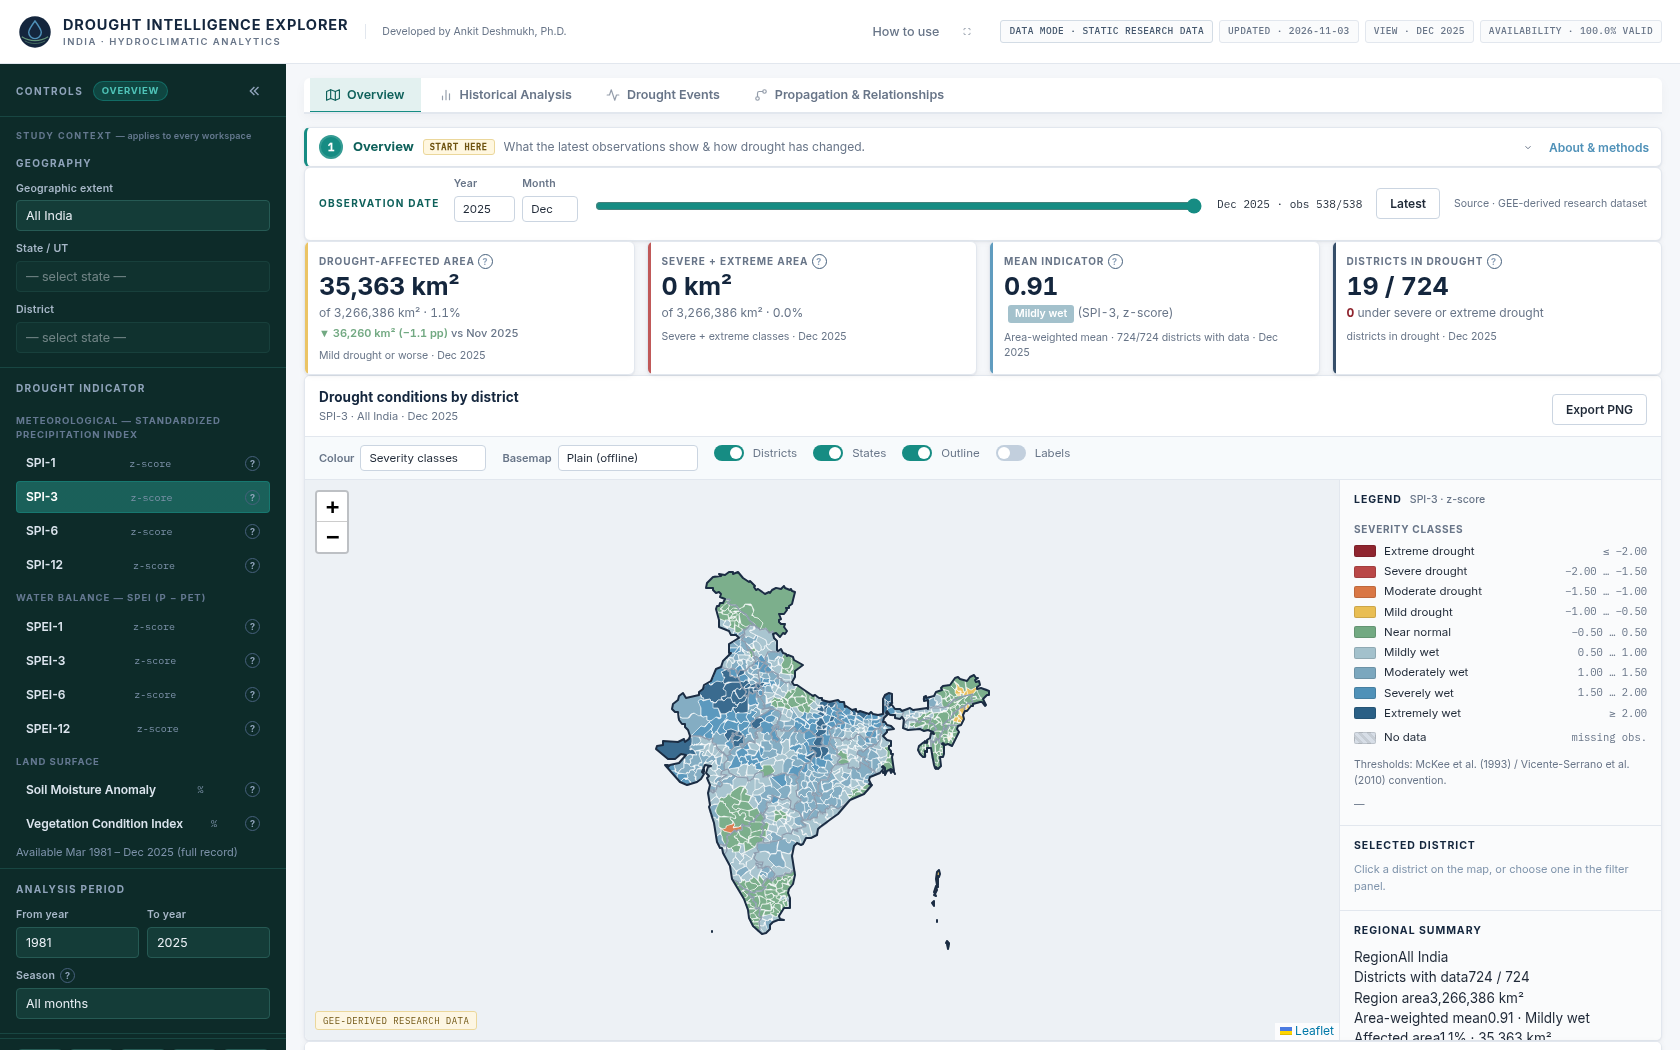
\includegraphics[width=\textwidth]{fig4_overview.png}
\caption{The Overview workspace of the live platform (\url{https://drought.ankitdeshmukh.com}, screenshot 2026-11-10) for SPI-3, All India, December 2025. The four KPI cards report the drought-affected area, the severe-plus-extreme subset, the area-weighted mean indicator with its severity class and the districts in drought, each with the change against the previous available observation; the choropleth classifies districts with the indicator's nine-class scheme; the legend, study-context sidebar, observation-date strip and provenance banner are visible.}
\label{fig:overview}
\end{figure}

\subsection*{Worked example 1: a current-conditions briefing}
Opening the Overview workspace with SPI-3 selected and the observation date set to December 2025 produces a one-page situational briefing (Figure~\ref{fig:overview}). Four KPI cards summarise the snapshot for All India: a drought-affected area of 35{,}363~km$^2$ (1.1\% of the 3{,}266{,}386~km$^2$ territory, in mild-or-worse classes), a severe-plus-extreme area of 0~km$^2$, an area-weighted mean indicator of 0.91 (mildly wet) computed over all 724 districts with data, and 19 of 724 districts in drought, none of them severe or worse; each card also shows the change against the previous available observation (November 2025). The choropleth classifies every district with the indicator's own nine-class scheme, hovering shows values and classes, and clicking a district focuses the whole application on it. The severity distribution panel decomposes the region's surface into classes, the ranking lists the ten most-affected districts with completeness flags, and the animated evolution timeline replays the share of area in drought across the entire 45-year record.

\subsection*{Worked example 2: historical characterisation and event forensics}
The Historical Analysis workspace quantifies frequency, duration, severity, trend and recurrence for any geography and analysis period (Figure~\ref{fig:historical}). For the All-India SPI-3 regional-mean series over 1981--2025, the panel reports four months at or below the $-1.00$ truncation level out of 538 valid months (0.7\%), namely July 1987 and July to September 2002, the two great national monsoon failures, with the series minimum of $-1.30$ in September 2002; these aggregate to one qualifying event. National averages mask district-level episodes (see Technical Validation, Table~\ref{tab:known}), which is precisely why the same panel provides per-district frequency histograms and duration and severity choropleths. The event catalogue in the Drought Events workspace (Figure~\ref{fig:events}) lists every per-district run with onset, termination, duration, maximum intensity, cumulative severity, recovery time and censoring flag, opens a detail view with the shaded event window on the district series, and re-computes all counts under alternative minimum-duration and truncation scenarios in the sensitivity panel. The trend panel completes the characterisation with the Mann--Kendall statistic, Sen's slope and its rank-based interval, applying and reporting the Hamed--Rao correction when the detrended series is significantly autocorrelated.

\begin{figure}[t]
\centering
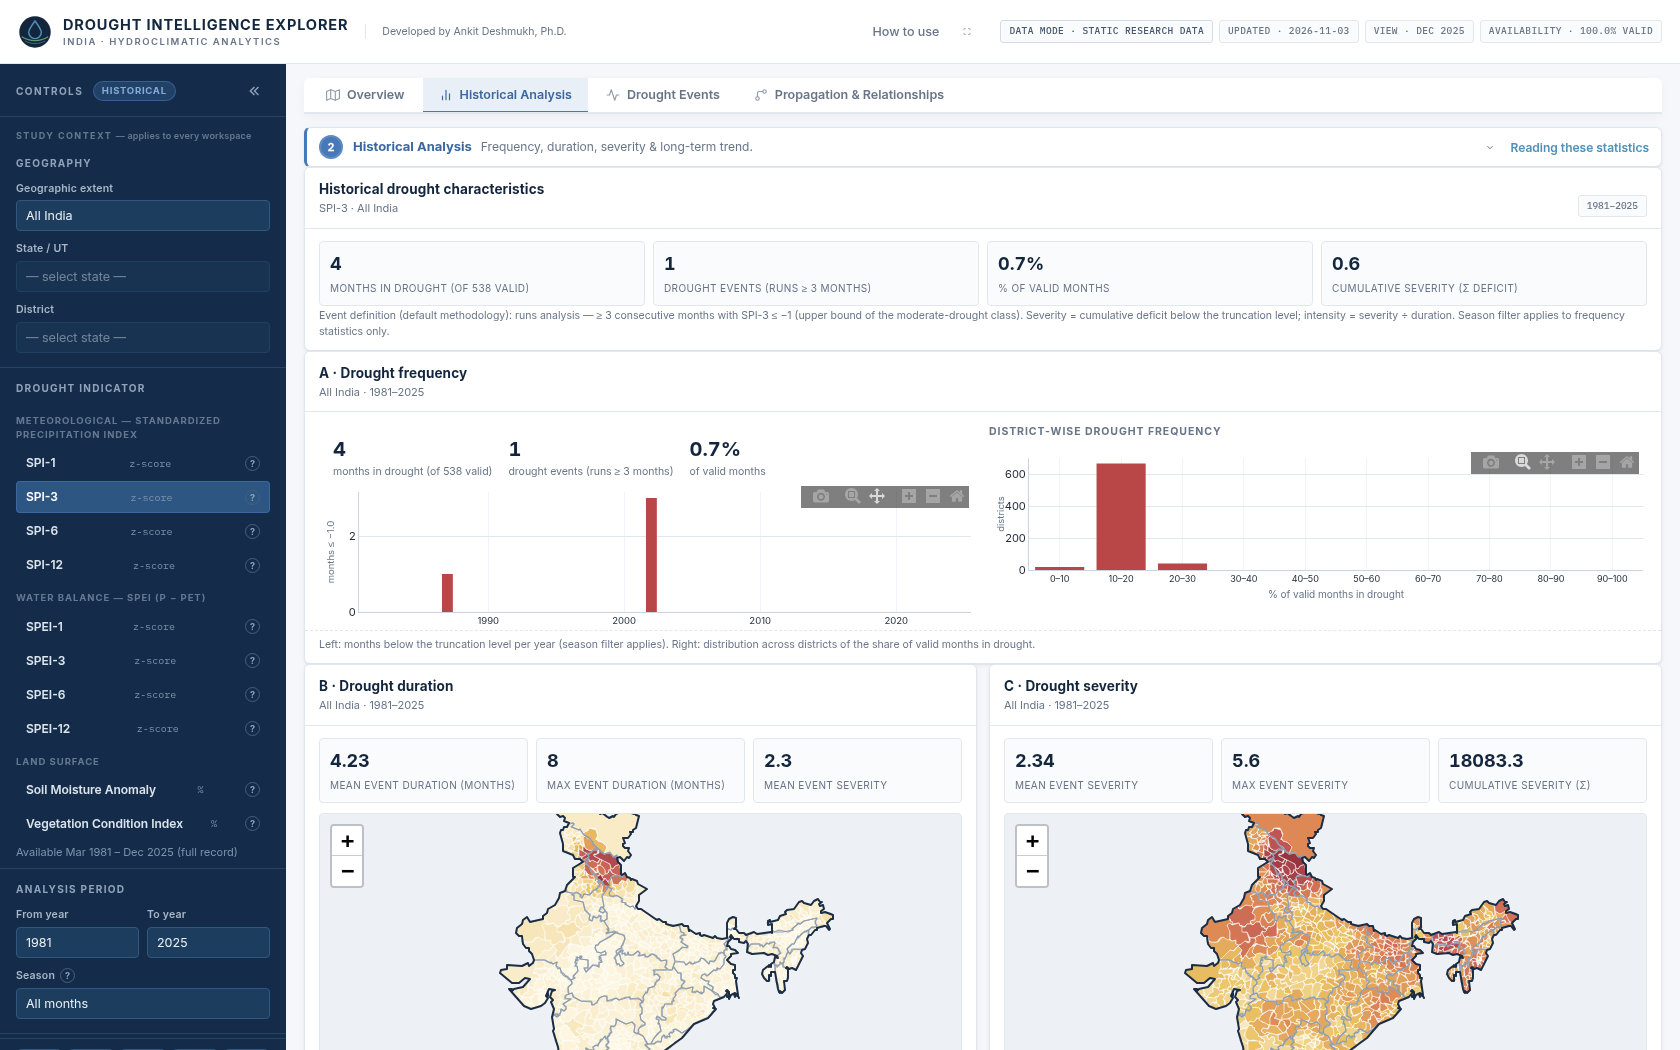
\includegraphics[width=\textwidth]{fig5_historical.png}
\caption{The Historical Analysis workspace for SPI-3, All India, 1981--2025 (screenshot 2026-11-10). The summary strip reports frequency statistics of the regional-mean series (4 months in drought of 538 valid months; 1 event under the default definition; cumulative regional severity 0.6); panels provide frequency by year, the district-wise frequency distribution, and per-district duration and severity statistics and maps, all computed with the documented event definition.}
\label{fig:historical}
\end{figure}

\subsection*{Worked example 3: indicator relationships and propagation}
The Propagation \& Relationships workspace quantifies how one indicator relates to another (Figure~\ref{fig:propagation}). The pairs that carry scientific meaning are the cross-family ones, in which a meteorological indicator leads a land-surface response; the results below are exploratory quantifications of association, not causal estimates of drought propagation. All figures are computed on the released matrices with the platform's own machinery: Pearson correlation at lags from $-12$ to $+12$ months on matched months, at least 30 matched pairs required, moving-block bootstrap with 1{,}000 resamples and fixed seed 20261103. Over the full lag window the All-India area-weighted SPI-3 series correlates most strongly with the SMA series at a lag of 0 months ($r=0.695$ over 538 matched months, 95\% CI $[0.617, 0.752]$) and with the VCI series (from February 2000) at a lag of 0 months ($r=0.576$ over 311 matched months, 95\% CI $[0.444, 0.661]$); no lag on either side of zero exceeds these values, so the search window does not manufacture the result. The association is synchronous at the monthly national scale but carries family-specific memory: the SPI-3--SMA correlation decays quickly with lag ($r=0.487$ at $+1$ month, $0.169$ at $+4$), whereas the SPI-3--VCI correlation decays slowly ($0.547$ at $+1$ month, $0.367$ at $+6$), consistent with soil moisture responding within the month and vegetation integrating the deficit over weeks to months. At district level (a simple random sample of 120 districts drawn with the release seed 20261103) the median optimal lag is 0 months, with median peak correlations of $+0.50$ for SPI-3 with SMA and $+0.36$ for SPI-3 with VCI; because neighbouring districts share the same climate, these district-level summaries are spatially dependent and should be read as indicative. The seasonal-scale sequencing behind the aggregates is visible in the 2015 Marathwada case of Technical Validation, where the September rainfall deficit is followed by the VCI minimum two to four months later. The by-construction pair shown in the interface demonstration, SPI-3 versus SPEI-3 (optimal lag 0 months, $r=0.874$, 95\% CI $[0.836, 0.902]$, $n=538$), is retained as a sanity anchor because two z-score families built from overlapping inputs must respond synchronously; the interface states explicitly that no association reported here is a causal claim. The $10\times10$ correlation heatmap shows every pair at its optimal lag while flagging the by-construction correlation of nested SPI/SPEI scales, and the district-wise optimal-lag map reveals where the response is longest. Streamflow and groundwater propagation are marked unavailable rather than simulated.

\begin{figure}[t]
\centering
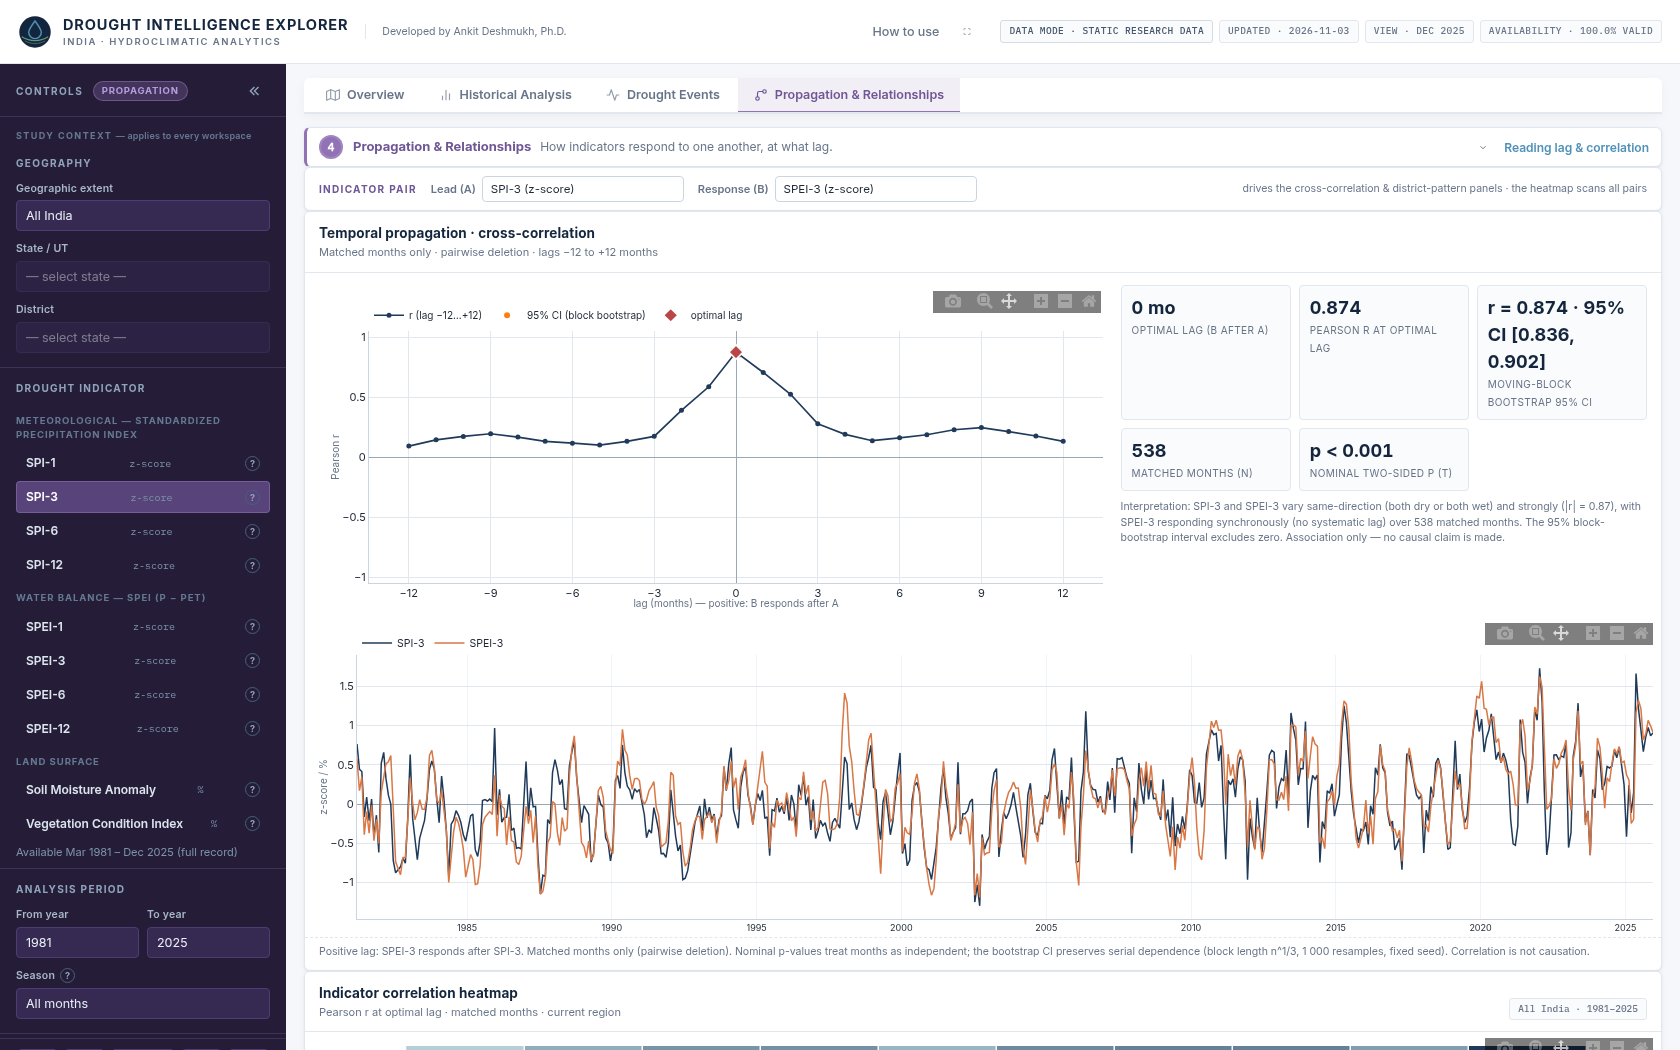
\includegraphics[width=\textwidth]{fig6_propagation.png}
\caption{The Propagation \& Relationships workspace (screenshot 2026-11-10): temporal cross-correlation of SPI-3 (lead) and SPEI-3 (response) over All India, 1981--2025, with the optimal lag (0 months), Pearson $r=0.874$ ($n=538$ matched months), the moving-block bootstrap 95\% confidence interval $[0.836, 0.902]$ (1{,}000 resamples, fixed seed) and the dual-series view. This by-construction pair is the interface's demonstration anchor; the cross-family propagation results (SPI-3 versus SMA and VCI) are reported in Worked example 3 and computed with the same machinery on the released matrices. The interface states the association-only interpretation and the cross-lag selection caveat.}
\label{fig:propagation}
\end{figure}

\begin{figure}[t]
\centering
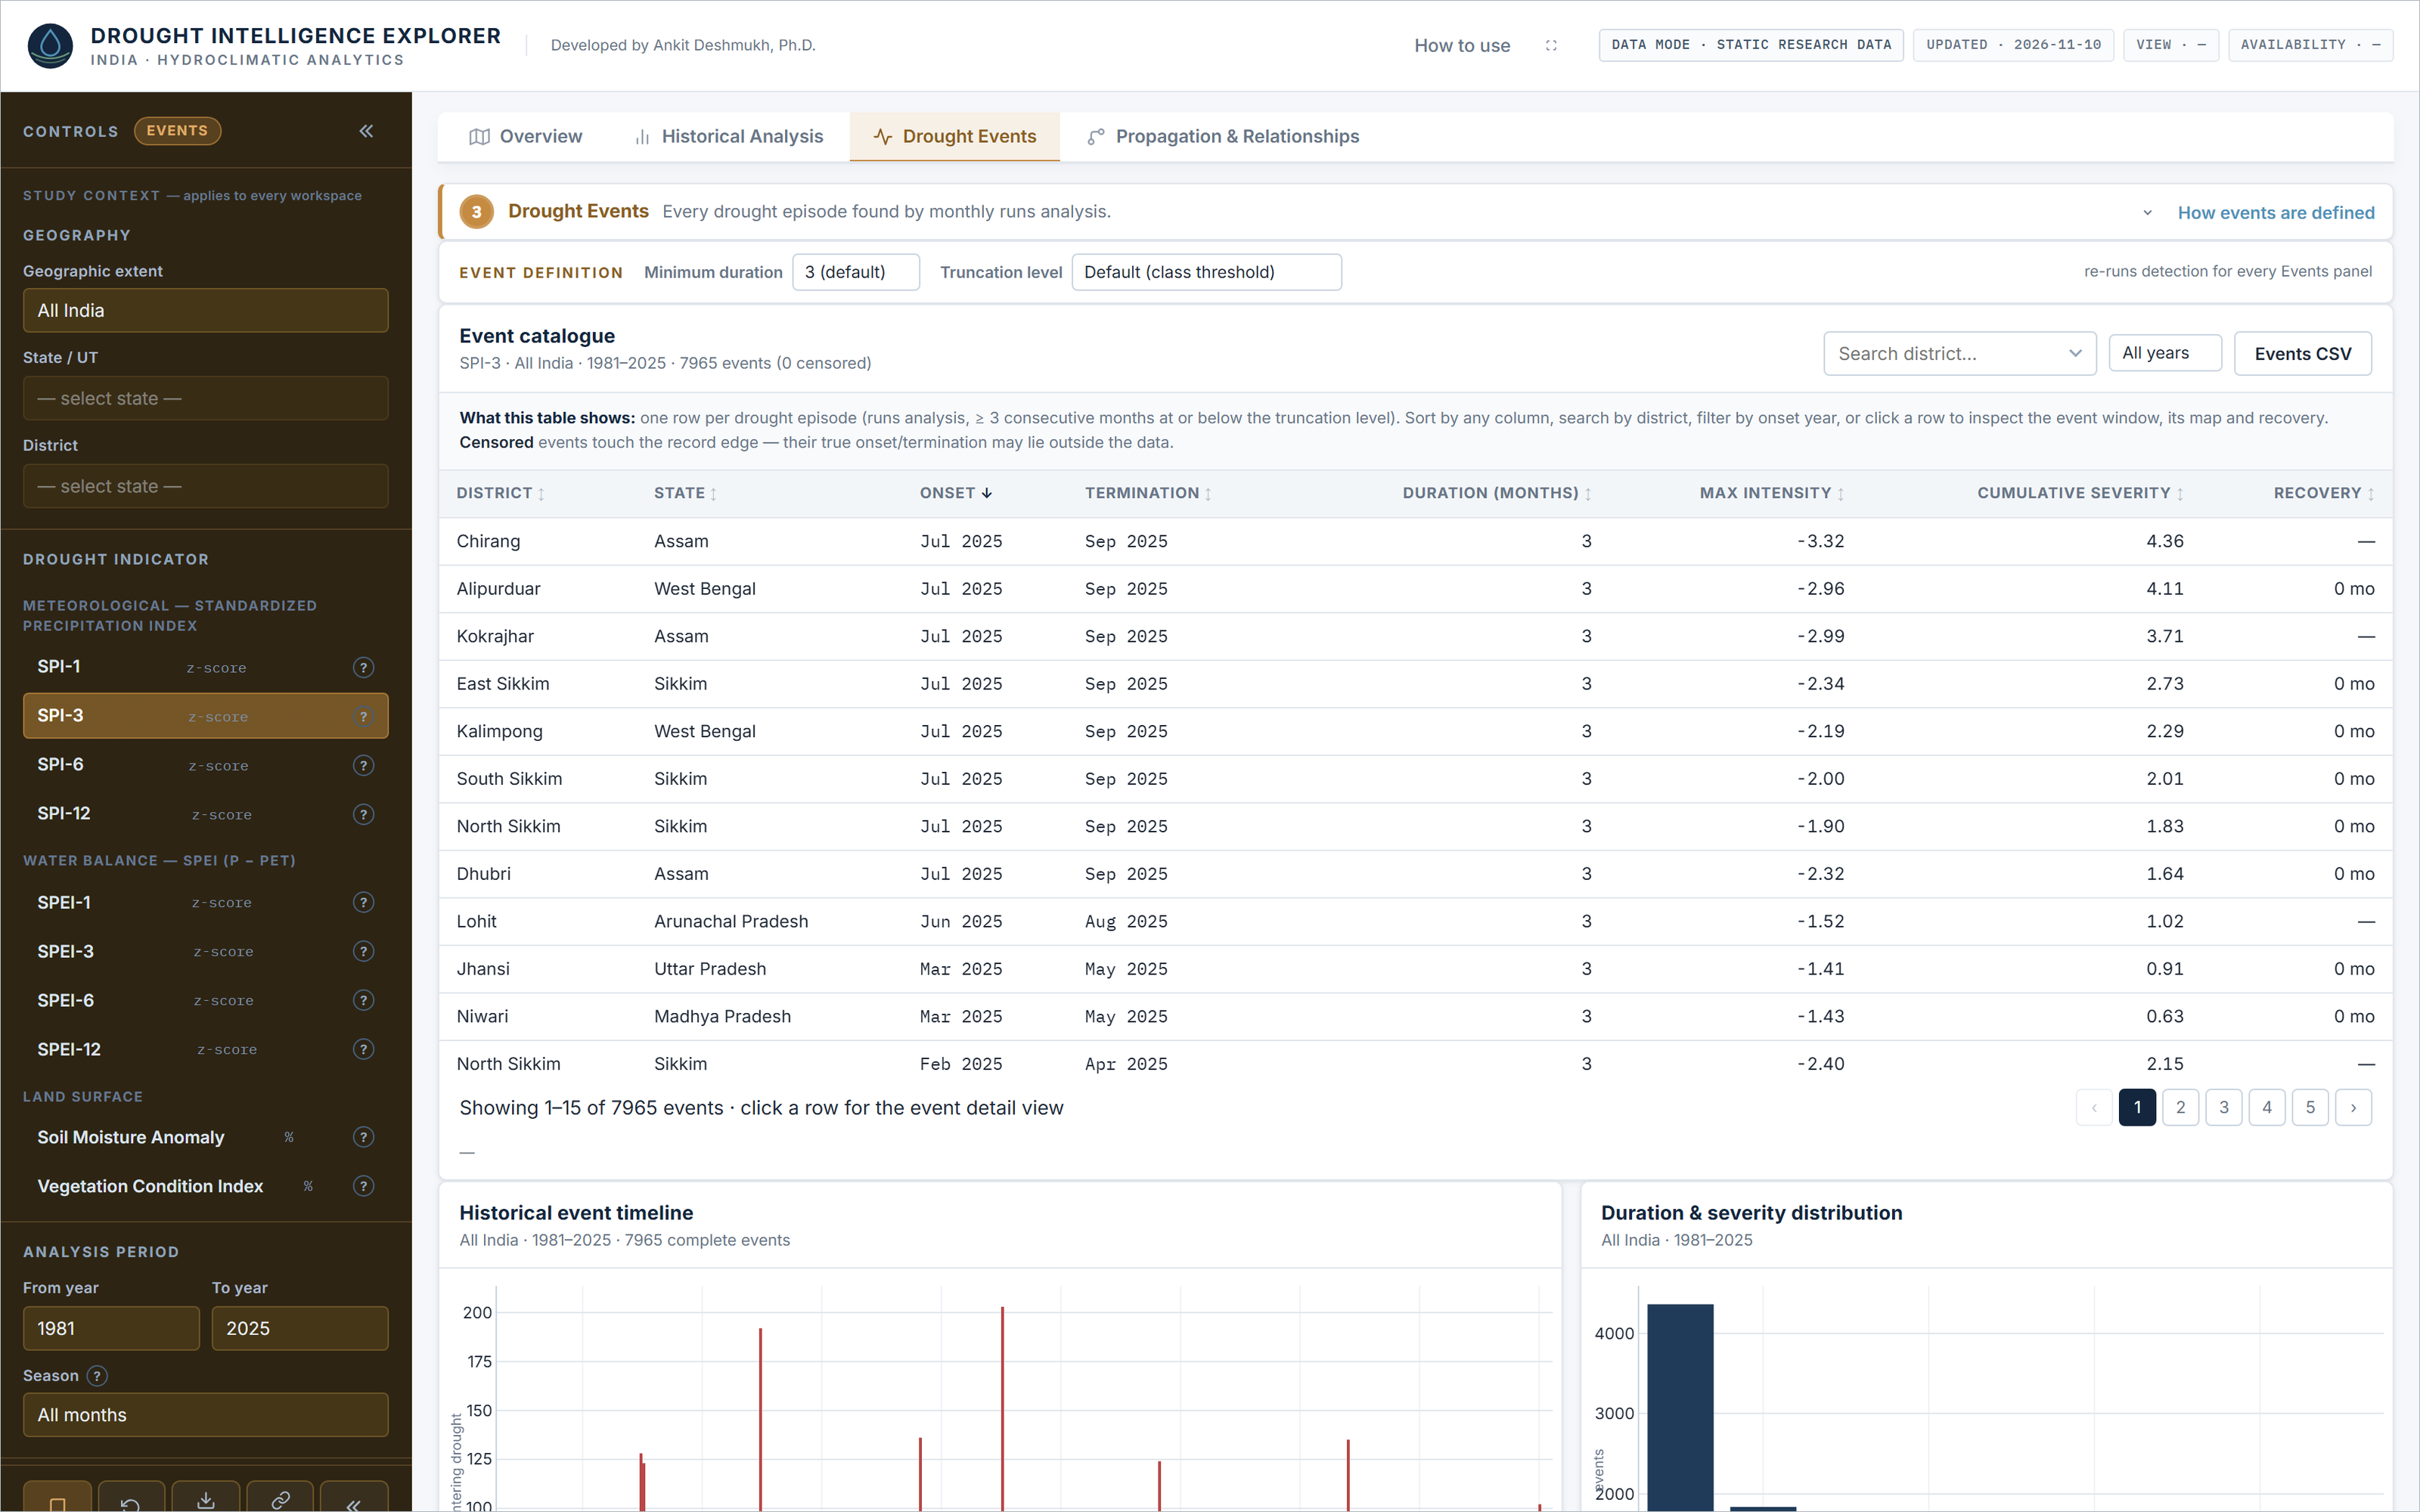
\includegraphics[width=\textwidth]{fig7_events.png}
\caption{The Drought Events workspace for SPI-3, All India, 1981--2025 (screenshot 2026-11-11). The event-definition strip (minimum duration, truncation level) re-runs detection for every Events panel when changed. The catalogue lists the district-level runs under the default definition (7,965 events, none censored at the record edges) with onset, termination, duration, maximum intensity, cumulative severity and recovery columns, searchable by district and filterable by onset year; each row opens an event detail view with the shaded event window on the district series. The historical timeline counts districts in drought per month, in which the two great national monsoon failures (July 1987 and July--September 2002) stand out, and the duration distribution shows the 3-month class as the most common event length.}
\label{fig:events}
\end{figure}

\subsection*{Guidance, inspection and responsive access}
The platform embeds its own explanation and verification surfaces, so that a first-time user can act correctly without external documentation (Figure~\ref{fig:guidance}). Clicking a district opens an inspection popup that reports the indicator value and severity class for the selected observation month, the district area and the record's data availability, and focuses every workspace on the selected district; the panel beside the map mirrors the selection. A \emph{How to use} guide opens from the header (or the question-mark shortcut) with a quick start, a per-workspace map of questions and outputs, and plain-language notes on reading the maps and KPI cards, uncertainty conventions and data caveats. The Documentation \& Resources area re-computes a load-time validation report in the browser --- completeness per indicator within its true availability window and structural checks (duplicate rows, invalid dates or values, identifier mismatches) --- with a one-click full audit that fetches the remaining matrices, and collects the download centre: wide and long-format CSVs, district and event statistics, cross-check files, the analysis-metadata JSON, boundary GeoJSON, the current map as PNG, the documentation in Markdown and a ready-to-paste citation with the release version history. The same interface is fully responsive: on phone-sized screens the study-context panel becomes a slide-in drawer, panels stack vertically, and the workspaces remain fully operable by touch (Figure~\ref{fig:responsive}); keyboard operation, visible focus states and ARIA roles serve the same accessibility goal on desktop.

\begin{figure}[t]
\centering
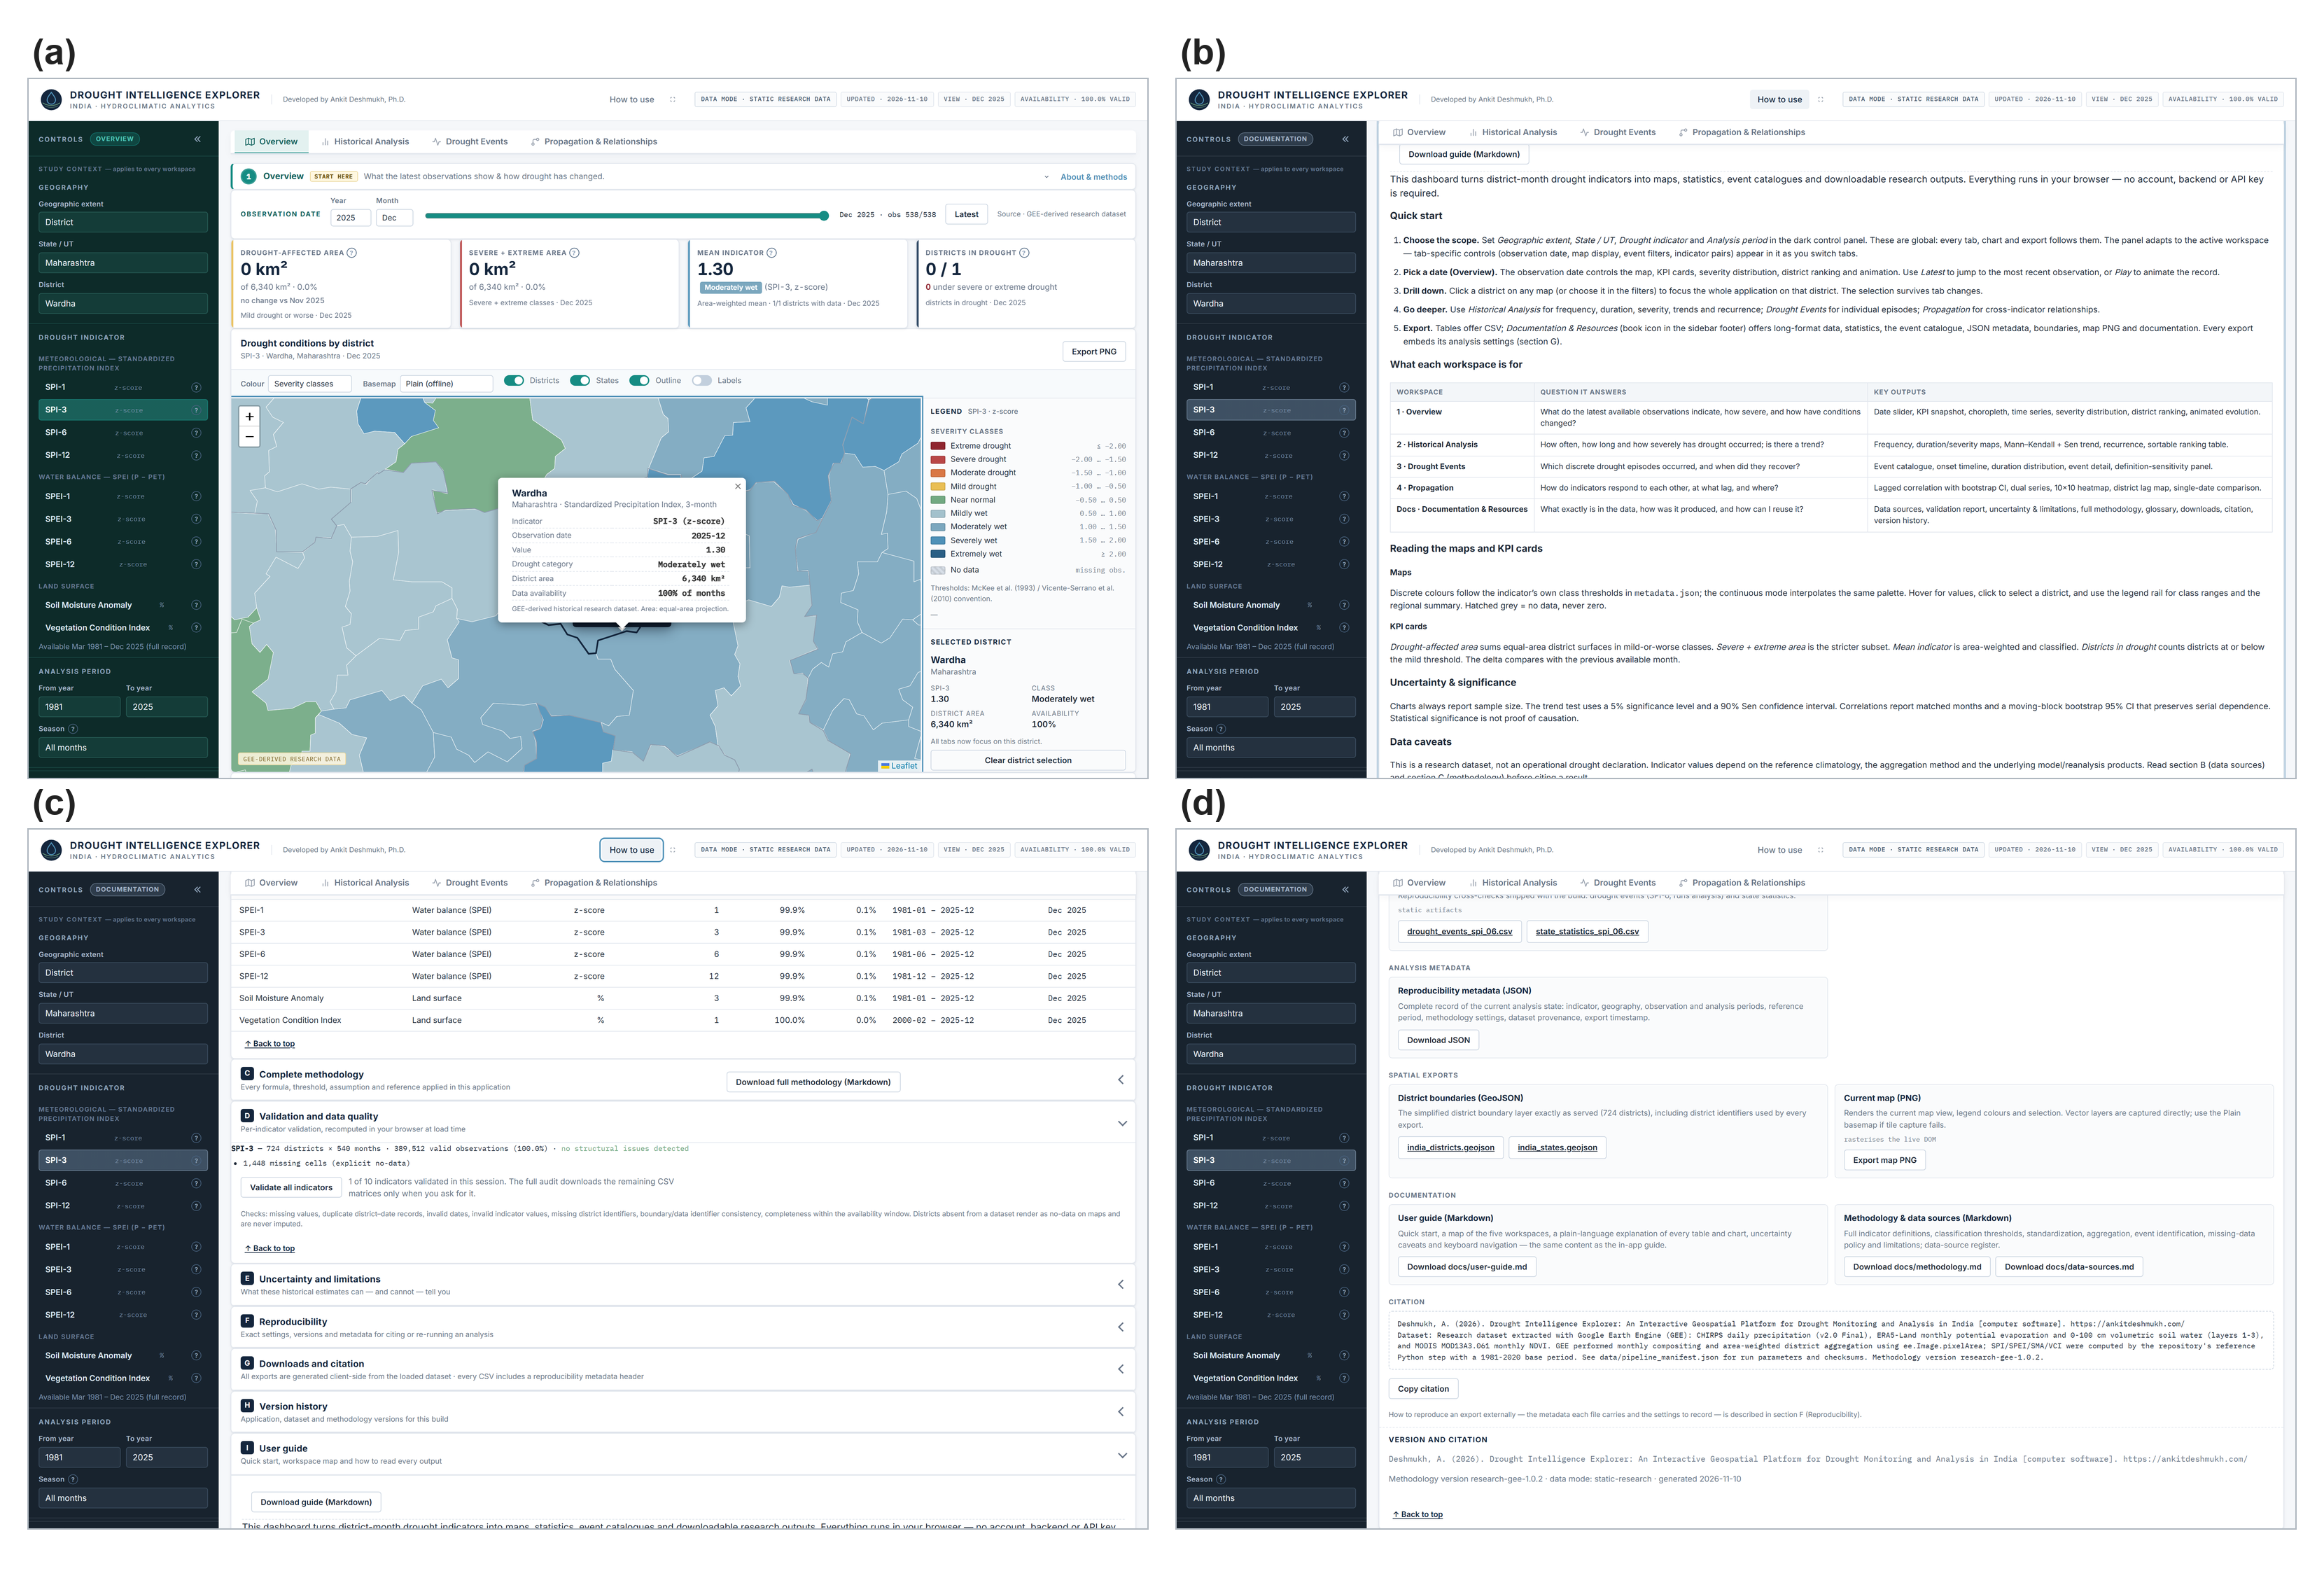
\includegraphics[width=\textwidth]{fig8_guidance.png}
\caption{Guidance, inspection and reproducibility surfaces (screenshot 2026-11-11, SPI-3, December 2025). (a)~Click-to-inspect popup for the Wardha district (Maharashtra): value $1.30$ (mildly wet), district category and area, $100\%$ data availability, with the nine-class legend and the selected-district panel; (b)~the integrated \emph{How to use} guide (quick start, workspace map, reading maps and KPI cards, uncertainty and caveats); (c)~the load-time validation report recomputed in the browser (per-indicator completeness and structural checks, here SPI-3 with $389{,}512$ valid district-months in its availability window --- $100.0\%$ --- plus $1{,}448$ explicit no-data cells from the 1981-01/02 accumulation warm-up) with the full-audit action; (d)~the download centre (cross-check CSVs, analysis-metadata JSON, boundary GeoJSON, map PNG, documentation downloads) with the ready-to-paste citation and version history.}
\label{fig:guidance}
\end{figure}

\begin{figure}[t]
\centering
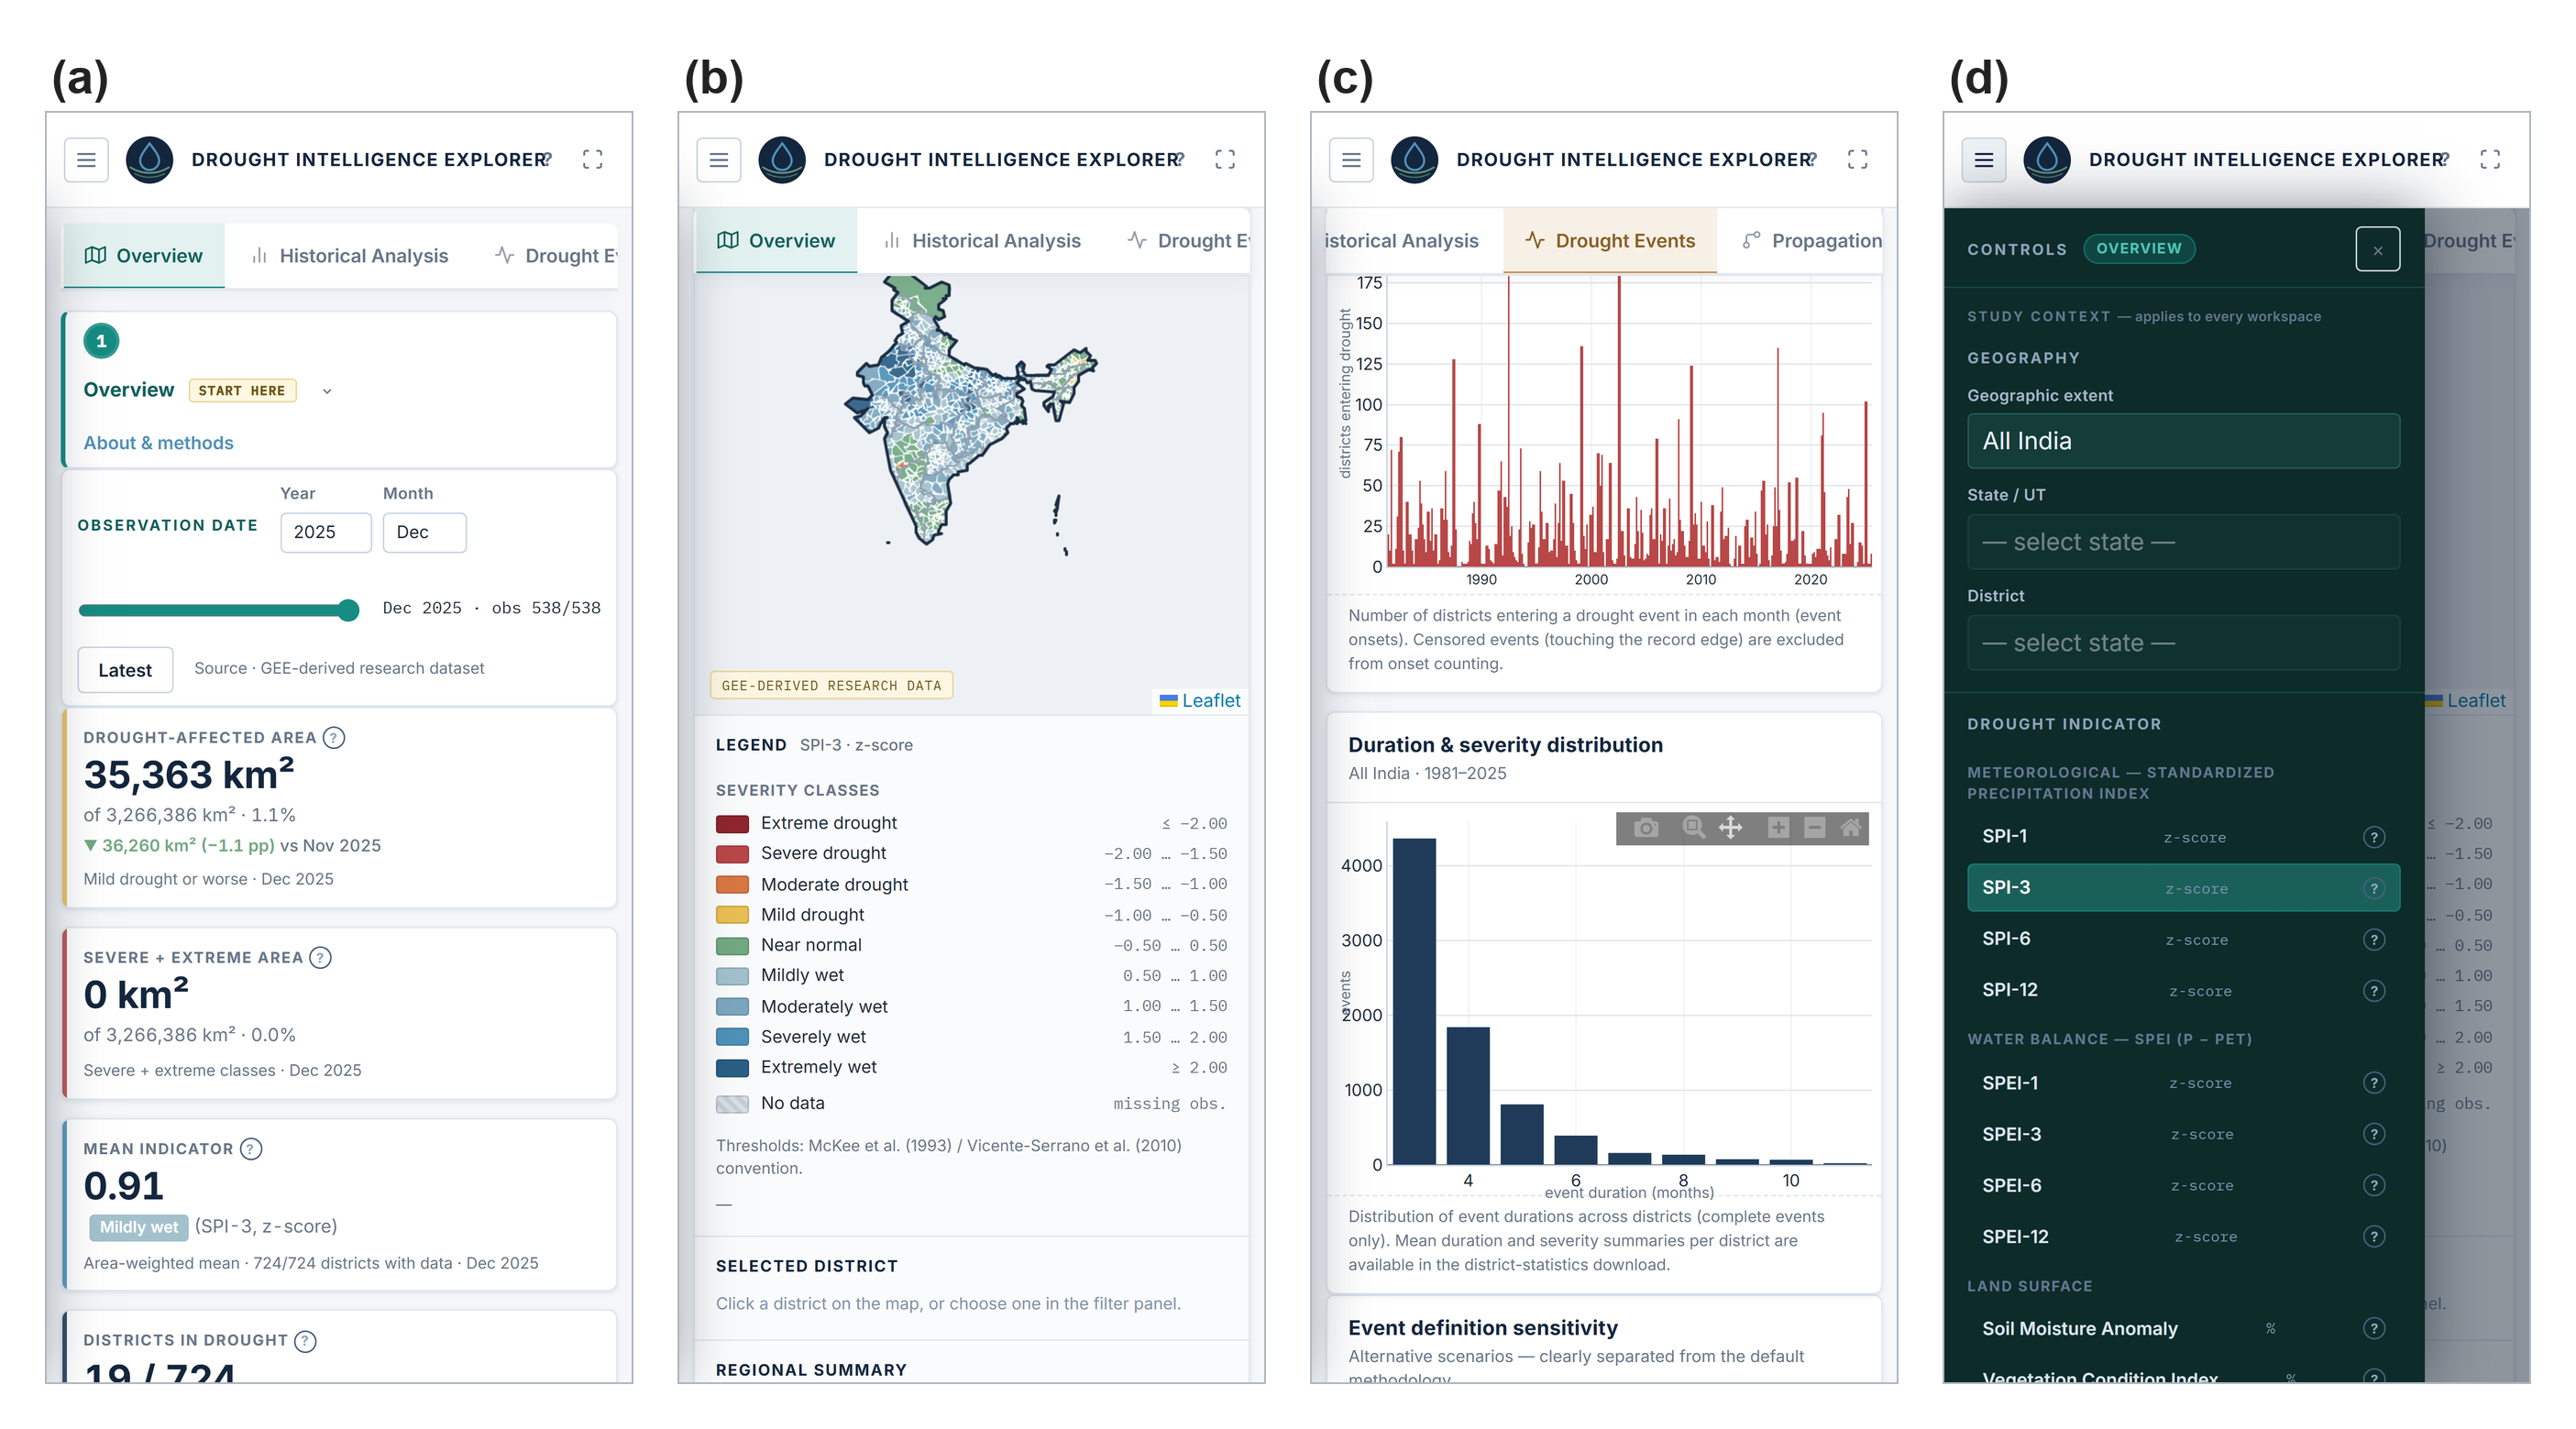
\includegraphics[width=\textwidth]{fig9_mobile.png}
\caption{The platform at phone size (390$\times$844 viewport, screenshot 2026-11-11). (a)~Overview: the KPI cards and observation-date strip stack vertically above the fold; (b)~the interactive district choropleth with its nine-class legend and display toolbar, fully operable by touch; (c)~Drought Events: the historical event timeline, the duration distribution and the definition-sensitivity panel; (d)~the study-context drawer (geography, indicator, analysis period) slides in over the workspace from the header toggle. No separate mobile application exists; the same static files serve every form factor.}
\label{fig:responsive}
\end{figure}

\subsection*{Exports and reproducible secondary analysis}
Ten export products are generated client-side: a long-format region extract (district-month rows with value, class, area and provenance), the exact distributed wide-format matrix, district drought statistics, the drought event catalogue, the current ranking table, an analysis-metadata JSON file that records the complete analysis state (indicator, geography, observation and analysis periods, reference period, methodology settings, seed and export time), boundary GeoJSON, the current map as PNG, the documentation, and a ready-to-paste citation. Every CSV begins with \texttt{\#} comment lines recording the indicator, geography, dataset and analysis periods, reference period, methodology version, data mode and seed, source and export timestamp, so the analysis settings travel with the numbers. A secondary analyst can therefore reproduce any figure of this paper by loading the exports into R or Python and applying the definitions of the Methods section, without re-deriving anything from the raw satellite record.

\section*{Reuse Potential}
For researchers, the record offers a district-level, multi-decadal, ten-indicator drought dataset for India together with a scripted pipeline that can be re-run for a new end date, modified spatial units or additional indicators using the same documented commands; the analytical tooling replaces what would otherwise be bespoke GIS and statistics work for every study. For the drought-methods community, the platform is a reference implementation of SPI and SPEI standardization with fit checking and fallback, runs-based event detection with censoring, Mann--Kendall/Sen testing with the Hamed--Rao correction, and moving-block bootstrap lag correlation, all visible in the interface with their caveats and exportable for independent verification. For practitioners and educators, zero-install access, the integrated methodology and glossary, and the worked caveats (censoring, reference-period dependence, correlation versus causation) make the platform usable for training as well as for situational analysis. For open science, the complete provenance chain from original observations through derived indicators to aggregated statistics, the versioned metadata, the fixed analysis seed, and the reproducibility headers on every export model transparent tool communication. The same architecture, a static data contract plus a metadata-driven front end, can be redeployed on other regions or newer datasets without code changes.

\section*{Version 1.0 scope and future updates}
This release is version~1.0 of both artefacts: dataset build \texttt{research-gee-1.0.2} (GEE extraction, 1981-01--2025-12, published 2026-11-10 with DOI 10.5281/zenodo.24113364) and platform release v1.0.0, which serves it. The scope of version~1.0 is deliberately bounded, ten indicators on a stable district fabric with a fully documented, validated, self-testable pipeline, because a citable, reproducible core is worth more than a broader but less auditable one. Every extension in Table~\ref{tab:roadmap} slots into the existing data contract without breaking compatibility: the metadata file already carries per-indicator availability windows, so adding an indicator or shortening a record is a data change, not a code change.

Planned future updates fall into five groups. \emph{Independent validation:} a quantitative comparison of CHIRPS-derived SPI against IMD gridded rainfall\citep{Pai2014,Srivastava2009} over a common period, reporting correlation, bias, root-mean-square difference and drought-class agreement, is the top priority, together with a Benjamini--Hochberg false-discovery-rate view in the trend maps. \emph{Input alignment:} the Earth Engine catalogue currently serves CHIRPS v2.0 while the offline route already targets v3.0; the GEE route will switch to v3.0 as soon as the catalogue mirrors it, eliminating the only version mismatch in the chain. \emph{Indicator breadth:} a sensitivity analysis of equal-weight versus thickness-weighted root-zone soil moisture; a fixed 2001--2020 VCI baseline as an alternative to the release-frozen baseline; a standardised (z-score) soil-moisture index, which exists as a configuration switch; change-point detection (for example the Pettitt test\citep{Pettitt1979}); and a multivariate composite index, clearly labelled as an analytical layer, not a replacement for the interpretable families\citep{HaoSingh2015}. \emph{Coverage and cadence:} scheduled rebuilds through continuous integration (the quarterly runbook and checksummed manifest already exist), versioned archival snapshots with a changelog, MODIS pixel-reliability screening, per-release recovery semantics for VCI, and extension to other regions; the pipeline is parameterised by bounding box, MODIS tile list and boundary file by design. \emph{Reach:} a multilingual interface (Hindi first) and sub-district aggregation, the latter only when a maintained geometry source makes it defensible. Streamflow and groundwater propagation remain unavailable until a public district-month observation source exists; the platform will keep stating that absence rather than simulating it.

\begin{table}[t]
\caption{Version 1.0 scope: planned future updates, what each would add, and its dependency.}
\label{tab:roadmap}
\footnotesize
\begin{tabularx}{\textwidth}{@{}p{0.24\textwidth}X p{0.26\textwidth}@{}}
\toprule
Planned addition & What it would add & Dependency / feasibility \\
\midrule
CHIRPS v3.0 on the GEE route & Version alignment between the two extraction routes & Pending Google catalogue update; offline route already on v3.0 \\
IMD gridded cross-validation & Independent national benchmark for SPI and SMA against IMD products\citep{Pai2014,Srivastava2009} & Data public; the known-event validation of this version (Table~\ref{tab:known}) is the first step, full IMD-series comparison follows \\
Standardised soil-moisture index & Distribution-free z-score alternative to percent-of-mean SMA & Configuration switch exists; class table remapping required \\
Change-point detection & Pettitt-type\citep{Pettitt1979} change-point statistics alongside trend tests & Client-side computation; low cost \\
Composite drought index & Joint-probability layer across families\citep{HaoSingh2015}, labelled as analytical & Methods established; kept optional and clearly flagged \\
Streamflow and groundwater & Observed hydrological-drought propagation & No public district-month source identified; stays unavailable rather than simulated \\
Seasonal outlook overlay & SEAS5/C3S anomaly context beside the historical record & C3S open data; analysis-only, never operational warning \\
Automated CI updates & Scheduled quarterly rebuild with validation gates & Runbook and manifest exist; credentials as repository secrets \\
Sub-district (block) units & Finer spatial aggregation & Requires a maintained geometry source; deferred \\
Multilingual interface & Hindi and State-language UI for practitioner reach & i18n of the static front end; low cost \\
Other regions & Same contract redeployed on new bounding boxes and boundaries & Pipeline is region-parameterised by design \\
Versioned archival snapshots & Per-release DOIs and a changelog in \texttt{metadata.json} & First versioned DOI minted (10.5281/zenodo.24113364); per-release workflow continues at updates \\
\bottomrule
\end{tabularx}
\end{table}

\section*{Limitations}
Six classes of limitation bound the use of this record, and the platform states them in the interface rather than leaving them to this section. First, the product is a historical and analytical explorer: it is not an operational or real-time monitoring system, and its values are model- and observation-based district aggregates that are not official drought declarations and not a substitute for India Meteorological Department or government bulletins. Second, spatial support: the indicators are district aggregates of gridded fields whose native resolutions are about 5~km (CHIRPS, $0.05^\circ$), 9--11~km (ERA5-Land, $0.1^\circ$) and 1~km (MODIS). District-level reporting does not change that resolution; a small district may share only a handful of source pixels with a larger one, so neighbouring small districts are not statistically independent, and the buffer fallback further changes the effective support for a few island units. The boundaries carry a 2011-era demarcation lineage, do not represent later reorganisations, and are not authoritative for legal purposes. Third, input and reanalysis uncertainty: the record inherits the biases of CHIRPS, ERA5-Land and MODIS and of their district aggregation. The PET used in SPEI is reanalysis potential evaporation, not a FAO-56 reference evapotranspiration, so SPEI here answers to a modelled evaporative demand rather than an agronomic one. The SMA is a reanalysis proxy for root-zone wetness, not observed soil moisture or hydrological drought. The VCI begins in 2000, and its min--max baseline depends on the release: values can shift slightly when a future release extends the record (see Indicator computation). The two water-balance indicators are absent for Lakshadweep because the ERA5-Land land mask carries no pixel there. Fourth, event statistics depend on the stated truncation level and minimum duration; the sensitivity panel quantifies but does not remove this dependence, and the recurrence statistics are empirical point estimates without fitted distributions, so they are indicative only. Recovery-to-neutral is meaningful for the signed families and is not reported for VCI (see Drought event identification). Fifth, the correlation machinery quantifies association, not causation; SPI and SPEI at nested accumulation windows correlate by construction, the confidence interval at the optimal lag is conditioned on that selection, and streamflow and groundwater propagation are unavailable because no such observations exist in the record. Sixth, statistical inference: the district-level Mann--Kendall trend maps are computed per district without adjustment for multiple testing (Technical Validation reports the scale of the issue and a demonstration correction), spatial dependence between neighbouring districts is not modelled, and because the reference climatology is fixed, indicator values after December 2020 are out-of-sample standardizations mapped through 1981--2020 parameters, which is the intended behaviour of a fixed climatology but bounds how the most recent years can be compared with the fitted period.

\section*{Data availability}
All indicator matrices, boundaries, registries, metadata and cross-check files described in Table~\ref{tab:records} are openly available in three coordinated locations: the archived release with the versioned DOI \href{https://doi.org/10.5281/zenodo.24113364}{10.5281/zenodo.24113364} (Zenodo, version 1.0.0, 2026-11-10), the public repository \url{https://github.com/anixn/drought-intelligence-explorer} at tag \texttt{v1.0.0}, and the live platform's Documentation \& Resources section at \url{https://drought.ankitdeshmukh.com} (data mode: static research, GEE-derived; methodology version \texttt{research-gee-1.0.2}; last updated 2026-11-10). Licences are stated per artefact. The software is released under the MIT licence on GitHub. The Zenodo archival record is published under the Creative Commons Attribution 4.0 International licence (CC BY 4.0), which covers reuse of the archived bundle. The indicator values are derived data; the original input products keep their own licences (CHIRPS public domain, ERA5-Land Copernicus licence with attribution, MOD13A3 NASA open data). The district boundaries come from the community-maintained india-maps-data repository (\url{https://github.com/udit-001/india-maps-data}, file \texttt{geojson/india.geojson}), accessed 2026-11-02 for the build and 2026-11-10 for the map figure of this paper. That source repository currently states no explicit redistribution licence; the boundaries are redistributed here with full attribution and the source's own disclaimer, the licence status is being confirmed with the maintainers before final publication, and the boundary layer is separable from the archived dataset so that it can be replaced without touching the indicators.

\section*{Code availability}
The complete processing pipeline (Google Earth Engine extraction, offline download route, indicator computation, boundary preparation with equal-area areas, export and validation) and the client-side application (vanilla JavaScript with Leaflet 1.9.4, PapaParse 5.4.1, Plotly-cartesian 2.35.2, Turf 7.2 and html2canvas 1.4.1; no build step) are released under the MIT licence at \url{https://github.com/anixn/drought-intelligence-explorer} (tag \texttt{v1.0.0}, released 2026-11-10) and archived with the dataset DOI \href{https://doi.org/10.5281/zenodo.24113364}{10.5281/zenodo.24113364}. The repository's \texttt{CITATION.cff} (cff-version 1.2.0) carries the machine-readable software citation, version, DOI, author ORCID (\href{https://orcid.org/0000-0002-1433-3872}{0000-0002-1433-3872}) and release date, and a dataset-type reference record for the indicator archive. The documented entry points are: \texttt{python run.py gee --project <project> --end 2025-12} (GEE extraction followed by indicators, export and validation), \texttt{python run.py update} (offline download, preparation, zonal statistics, indicators, export, validation), \texttt{python run.py indicators / export / validate} (individual shared stages), \texttt{python run.py status} (inventory of raw, processed and released data), \texttt{python selftest.py} (offline end-to-end test; 82 seed-deterministic assertions), and \texttt{python prepare\_boundaries.py} (simplification and equal-area areas). A verification script released alongside the pipeline reproduces the statistical evidence quoted in Methods and Technical Validation (L-moment parameter recovery, the small-sample MLE wet bias at $n=40$ in the SPEI simulation, tie handling of the Gringorten transform, classification continuity, the area-weighting accuracy of the aggregation, and the Benjamini--Hochberg trend demonstration), so every quantified methodological claim in this paper is checkable by running one script. The shipped \texttt{config.yaml} exposes every scientific parameter (base periods, minimum base years, valid ranges, indicator definitions, QA thresholds and dataset mappings) with no hidden constants in code.

\section*{Acknowledgements}
The author thanks the Climate Hazards Center at the University of California, Santa Barbara for CHIRPS; the Copernicus Climate Change Service and ECMWF for ERA5-Land; NASA LP DAAC and the MODIS science teams for MOD13A3; the Google Earth Engine team for the extraction infrastructure; and the maintainers of the community India district boundaries dataset. No external funding was received for this work.

\section*{Author contributions}
A.D. designed and built the dataset and pipeline, implemented the platform and its analytical machinery, designed the validation and reproducibility framework, and wrote the manuscript.

\section*{Competing interests}
The author declares no competing interests.

% =====================================================================
\begin{thebibliography}{31}
\footnotesize

\bibitem[Beguer\'{\i}a et~al.(2014)]{Begueria2014} Beguer\'{\i}a, S., Vicente-Serrano, S.~M., Reig, F. \& Latorre, B. Standardized precipitation evapotranspiration index (SPEI) revisited: parameter fitting, probabilistic inference and information-based model selection. \textit{Environ. Model. Softw.} \textbf{69}, 105--119 (2014).

\bibitem[Deshmukh(2026)]{Deshmukh2026} Deshmukh, A. \textit{Drought Intelligence Explorer: an interactive geospatial platform for drought monitoring and analysis in India}, version 1.0.0 [computer software, methodology version \texttt{research-gee-1.0.2}] (2026). \url{https://github.com/anixn/drought-intelligence-explorer}; \href{https://doi.org/10.5281/zenodo.24113364}{doi:10.5281/zenodo.24113364}

\bibitem[Didan(2015)]{Didan2015} Didan, K. \textit{MOD13A3 MODIS/Terra Vegetation Indices Monthly L3 Global 1 km SIN Grid V061} (NASA EOSDIS Land Processes DAAC, 2015).

\bibitem[Funk et~al.(2015)]{Funk2015} Funk, C. \textit{et al.} The climate hazards infrared precipitation with stations: a new environmental record for monitoring extremes. \textit{Sci. Data} \textbf{2}, 150066 (2015).

\bibitem[Gadgil and Gadgil(2006)]{GadgilGadgil2006} Gadgil, S. \& Gadgil, S. The Indian monsoon, GDP and agriculture. \textit{Econ. Polit. Wkly.} \textbf{41}, 4887--4895 (2006).

\bibitem[Gilbert(1987)]{Gilbert1987} Gilbert, R.~O. \textit{Statistical Methods for Environmental Pollution Monitoring} (Van Nostrand Reinhold, 1987).

\bibitem[Gorelick et~al.(2017)]{Gorelick2017} Gorelick, N., Hancher, M., Dixon, M., Ilyushchenko, S., Thau, D. \& Moore, R. Google Earth Engine: planetary-scale geospatial analysis for everyone. \textit{Remote Sens. Environ.} \textbf{202}, 18--27 (2017).

\bibitem[Gringorten(1963)]{Gringorten1963} Gringorten, I.~I. A plotting rule for extreme probability paper. \textit{J. Geophys. Res.} \textbf{68}, 813--814 (1963).

\bibitem[Hamed and Rao(1998)]{HamedRao1998} Hamed, K.~H. \& Rao, A.~R. A modified Mann--Kendall trend test for autocorrelated data. \textit{J. Hydrol.} \textbf{204}, 182--196 (1998).

\bibitem[Hao and Singh(2015)]{HaoSingh2015} Hao, Z. \& Singh, V.~P. Drought characterization from a multivariate perspective: a review. \textit{J. Hydrol.} \textbf{527}, 668--678 (2015).

\bibitem[Hersbach et~al.(2020)]{Hersbach2020} Hersbach, H. \textit{et al.} The ERA5 global reanalysis. \textit{Q. J. R. Meteorol. Soc.} \textbf{146}, 1999--2049 (2020).

\bibitem[Hosking(1990)]{Hosking1990} Hosking, J.~R.~M. L-moments: analysis and estimation of distributions using linear combinations of order statistics. \textit{J. R. Stat. Soc. B} \textbf{52}, 105--124 (1990).

\bibitem[Kendall(1975)]{Kendall1975} Kendall, M.~G. \textit{Rank Correlation Methods}, 4th edn (Charles Griffin, 1975).

\bibitem[Kogan(1995)]{Kogan1995} Kogan, F.~N. Application of vegetation index and brightness temperature for drought detection. \textit{Adv. Space Res.} \textbf{15}, 91--100 (1995).

\bibitem[K\"{u}nsch(1989)]{Kunsch1989} K\"{u}nsch, H.~R. The jackknife and the bootstrap for general stationary observations. \textit{Ann. Stat.} \textbf{17}, 1217--1241 (1989).

\bibitem[Mallya et~al.(2016)]{Mallya2016} Mallya, G., Mishra, V., Niyogi, D., Tripathi, S. \& Govindaraju, R.~S. Trends and variability of droughts over the Indian monsoon region. \textit{Weather Clim. Extremes} \textbf{12}, 43--68 (2016).

\bibitem[Mann(1945)]{Mann1945} Mann, H.~B. Nonparametric tests against trend. \textit{Econometrica} \textbf{13}, 245--259 (1945).

\bibitem[McKee et~al.(1993)]{McKee1993} McKee, T.~B., Doesken, N.~J. \& Kleist, J. The relationship of drought frequency and duration to time scales. In \textit{Proc. 8th Conference on Applied Climatology} 179--184 (American Meteorological Society, 1993).

\bibitem[Mishra and Singh(2010)]{MishraSingh2010} Mishra, A.~K. \& Singh, V.~P. A review of drought concepts. \textit{J. Hydrol.} \textbf{391}, 202--216 (2010).

\bibitem[Mu\~{n}oz-Sabater et~al.(2021)]{MunozSabater2021} Mu\~{n}oz-Sabater, J. \textit{et al.} ERA5-Land: a state-of-the-art global reanalysis dataset for land applications. \textit{Earth Syst. Sci. Data} \textbf{13}, 4349--4383 (2021).

\bibitem[Pai et~al.(2014)]{Pai2014} Pai, D.~S., Sridhar, L., Rajeevan, M., Sreejith, O.~P., Satbhai, N.~S. \& Mukhopadhyay, B. Development of a new high spatial resolution ($0.25^\circ\times0.25^\circ$) long period (1901--2010) daily gridded rainfall data set over India. \textit{Mausam} \textbf{65}, 1--18 (2014).

\bibitem[Pettitt(1979)]{Pettitt1979} Pettitt, A.~N. A non-parametric approach to the change-point problem. \textit{J. R. Stat. Soc. C} \textbf{28}, 126--135 (1979).

\bibitem[Sen(1968)]{Sen1968} Sen, P.~K. Estimates of the regression coefficient based on Kendall's tau. \textit{J. Am. Stat. Assoc.} \textbf{63}, 1379--1389 (1968).

\bibitem[Smith et~al.(2016)]{Smith2016} Smith, J.~P. \textit{et al.} An expandable web-based platform for visually analyzing basin-scale hydro-climate time series data. \textit{Environ. Model. Softw.} \textbf{78}, 97--105 (2016).

\bibitem[Srivastava et~al.(2009)]{Srivastava2009} Srivastava, A.~K., Rajeevan, M. \& Kshirsagar, S.~R. Development of a high resolution daily gridded temperature data set (1969--2005) for the Indian region. \textit{Atmos. Sci. Lett.} \textbf{10}, 249--254 (2009).

\bibitem[Stagge et~al.(2015)]{Stagge2015} Stagge, J.~H., Tallaksen, L.~M., Gudmundsson, L., Van Loon, A.~F. \& Stahl, K. Candidate distributions for climatological drought indices (SPI and SPEI). \textit{Int. J. Climatol.} \textbf{35}, 4027--4040 (2015).

\bibitem[Svoboda and Fuchs(2016)]{SvobodaFuchs2016} Svoboda, M. \& Fuchs, B.~A. \textit{Handbook of Drought Indicators and Indices} (World Meteorological Organization / Global Water Partnership, Integrated Drought Management Programme, 2016).

\bibitem[Vicente-Serrano et~al.(2010)]{VicenteSerrano2010} Vicente-Serrano, S.~M., Beguer\'{\i}a, S. \& L\'{o}pez-Moreno, J.~I. A multiscalar drought index sensitive to global warming: the Standardized Precipitation Evapotranspiration Index. \textit{J. Clim.} \textbf{23}, 1696--1718 (2010).

\bibitem[Wilhite and Glantz(1985)]{WilhiteGlantz1985} Wilhite, D.~A. \& Glantz, M.~H. Understanding the drought phenomenon: the role of definitions. \textit{Water Int.} \textbf{10}, 111--120 (1985).

\bibitem[WMO(2009)]{WMOLincoln2009} World Meteorological Organization. \textit{Inter-regional Workshop on Indices and Early Warning Systems for Drought: Lincoln Declaration on Drought Indices} (WMO, 2009).

\bibitem[Yevjevich(1967)]{Yevjevich1967} Yevjevich, V. \textit{An Objective Approach to Definitions and Investigations of Continental Hydrologic Droughts}, Hydrology Papers No.~23 (Colorado State University, 1967).

\end{thebibliography}

\end{document}
